\chapter[Mina]{Mina}
\label{ch:mina}

Este capítulo compreende a apresentação do aplicativo Mina, desenvolvido ao longo desse trabalho. 
Com esse intuito, tem-se uma breve contextualização sobre a ideia do trabalho, seguido dos 
detalhamentos quanto: à coleta de dados; requisitos; arquitetura, e aplicativo em si. Por fim, 
têm-se as considerações finais do capítulo.

A ideia sobre o domínio ciclo menstrual e atividades surgiu a 
partir de um video\footnote{video :https://www.youtube.com/watch?v=sNRi9A6LaHM. Último acesso em: 03/12/2020}, 
em que a palestrante comenta sobre um 
trabalho que ela estava desenvolvendo com mais duas  
mulheres, e que elas gerenciaram o projeto, delegando tarefas, de 
acordo com o ciclo menstrual de cada uma. Levantam a hipótese de 
que em cada fase do ciclo menstrual, cada mulher tem um tipo 
de comportamento e por isso, nessas fases, algumas atividades 
podem ser mais produtivas.
A própria autora deste trabalho começou a notar então, na sua 
vivência, que certos padrões se repetiam, ciclo após ciclo.

Essa inspiração foi levada aos 
orientadores, e começaram a ser discutidas possíveis aplicações da 
engenharia de software sobre o domínio. Duas ideias centrais 
foram identificadas. 

A primeira ideia foi utilizar aprendizado de máquina para 
acordar um perfil comportamental com base no ciclo menstrual e, 
com isso, conferir previsões sobre produtividade, humor, sintomas 
físicos, entre outros. Essa ideia foi descartada porque, para 
um bom desempenho de um aprendizado de máquina, seria necessário 
uma base de dados volumosa, dados esses que 
a autora não continha. Além disso, o termo produtividade também 
foi descartado por envolver uma medida muito subjetiva e questões éticas e morais. 

A segunda ideia surgiu baseada no trabalho de \citeonline{leticia}, Sistema de Recomendação para Atribuição de Tarefas de Testes 
Baseado em Perfil de Testadores. Foi considerado o fato de que, seria 
possível desenvolver um tema similar, só que no
contexto de recomendações de tarefas baseadas no perfil e 
ciclo menstrual. A segunda ideia foi a escolhida para ser 
utilizada para o desenvolvimento deste trabalho.

Algumas problemáticas sobre o tema foram levantadas. A primeira 
foi: o trabalho vai contar com o acompanhamento de um 
profissional da área da saúde? Optou-se por não envolver 
terceiros no desenvolvimento do trabalho, devido à dificuldade em encontrar uma pessoa 
com disponibilidade e interesse em 
acompanhar o projeto. A segunda problemática foi: 
como adquirir os dados necessários para desenvolver um 
Sistema de Recomendação? Optou-se por criar um grupo específico que serviu como
estudo de caso, participando tanto 
da coleta de dados, quanto dos testes da aplicação. O estudo de 
caso também resolveu, de certa forma, a primeira problemática, 
porque delimitou o desenvolvimento da aplicação para um grupo 
específico de pessoas.


\section{Coleta de Dados}
\label{coletadados}

Um grupo com 23 mulheres que se interessaram pelo tema foi criado durante a execução da primeira etapa do TCC. 
As mulheres participantes do grupo são jovens entre 20 a 35 anos, e possuem 
formação acadêmica ou estão em formação, caracterizando pessoas bem instruídas e com um bom 
nível de acesso à informação.

A primeira atividade com o grupo envolveu discussões de como as colaboradoras se sentiam durante as fases. Foi orientado
às participantes que ficassem mais atentas às mudanças e como elas influenciavam na realização de 
atividades cotidianas. Para que elas se sentissem mais confortáveis realizando a tarefa, o método para tomar notas ficou a cargo de cada uma. 
Algumas começaram a anotar em uma agenda, e outras utilizaram 
aplicativos de ciclo menstrual já existentes no mercado. Ficou acordado que, 
nesse momento, as notas não precisam ser compartilhadas e que, posteriormente, o grupo seria aberto para 
aquelas que se sentissem confortáveis em compartilhar o que perceberam 
durante esse trabalho interno.

As discussões com o grupo e o estudo inicial da referência bibliográfica foram então utilizadas para 
delimitar questões que seriam aplicadas à primeira coleta de dados, a partir de um questionário.

\subsection{Definição da Plataforma}

Após expor ao grupo o tema do trabalho, foi realizada uma enquete para definir que tipo de plataforma as 
integrantes preferiam para o desenvolvimento da aplicação. A Figura \ref{fig07} traz o resultado da enquete. 
Ficou definido, então, que seria um aplicativo.

\begin{figure}[ht]
	\caption{Enquete Sobre a Aplicação}
	\begin{center}
	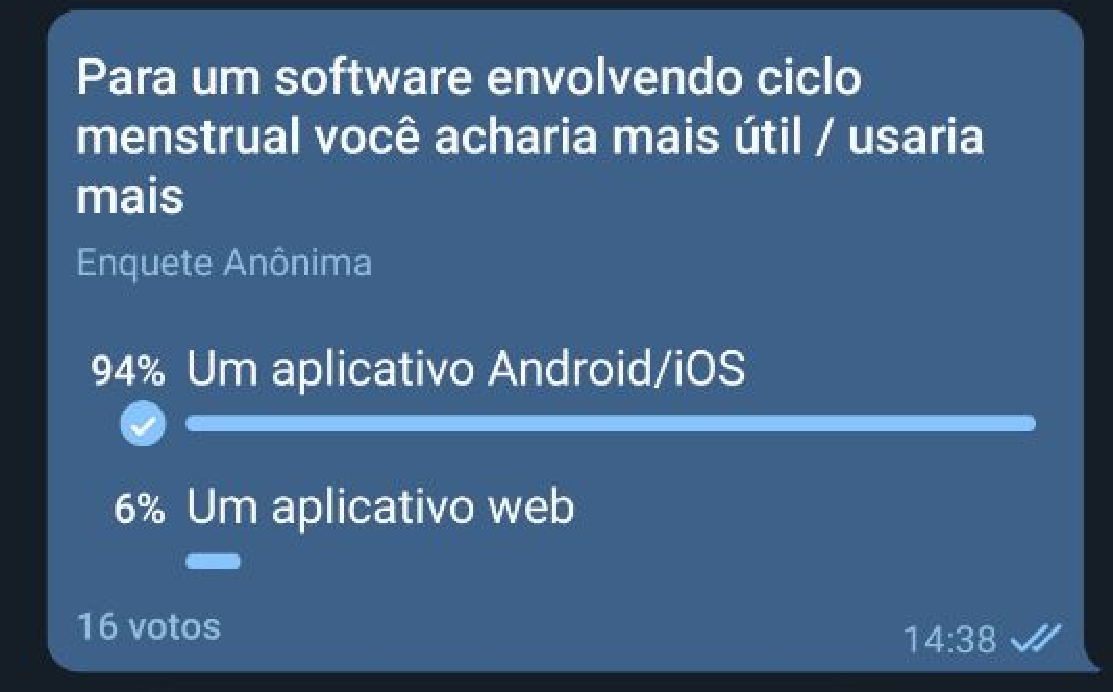
\includegraphics[keepaspectratio=true,scale=0.3]{figuras/enqueteApp.pdf}
	\end{center}
	\legend{Fonte: Autora}
    \label{fig07}
\end{figure}

\subsection{Primeiro Questionário}

A Tabela \ref{tab07} e a Tabela \ref{tab08} apresentam as questões que foram utilizadas para o primeiro ciclo de coleta de dados sobre o ciclo menstrual e 
sua influência. O questionário\footnote{segundo questionário : https://forms.gle/4Q3HoyXydcY89TjY9} foi feito utilizando a plataforma Google Forms, sendo respondido de forma anônima, para que as
participantes se sentissem mais confortáveis respondendo-o. Ao todo, o questionário contou com 31 perguntas, sendo 20 fechadas e 
11 abertas. Foram recebidas 23 respostas até a data 18/03/2020.

\begin{table}[ht]
    \centering
    \caption{Perguntas Fechadas do Questionário}
    \label{tab07}
    \begin{tabular}{c}
        \toprule
        \textbf{Perguntas fechadas} \\
        \midrule
        \begin{minipage} [t] {1\textwidth} Qual a sua idade?  \end{minipage} \\
        \midrule
        \begin{minipage} [t] {1\textwidth} Você utiliza algum método contraceptivo hormonal?   \end{minipage}\\
        \midrule
        \begin{minipage} [t] {1\textwidth} Você utiliza algum método contraceptivo não hormonal?  \end{minipage} \\
        \midrule
        \begin{minipage} [t] {1\textwidth}  Você tem algum distúrbio endócrino como ovários policísticos? Ou outros? \end{minipage}  \\
        \midrule
        \begin{minipage} [t] {1\textwidth}  Você monitora o seu ciclo? \end{minipage}\\
        \midrule
        \begin{minipage} [t] {1\textwidth}  Como você monitora o seu ciclo? \end{minipage} \\
        \midrule
        \begin{minipage} [t] {1\textwidth}  Você iria preferir uma aplicação para monitorar o seu ciclo?\end{minipage}\\
        \midrule
        \begin{minipage} [t] {1\textwidth}  Qual o tamanho do seu ciclo? \end{minipage}\\
        \midrule
        \begin{minipage} [t] {1\textwidth}  Você sente que de alguma forma seu ciclo influencia sua produtividade em certas atividades do dia-a-dia? \end{minipage}\\
        \midrule
        \begin{minipage} [t] {1\textwidth}  Em uma escala de 0 a 4 o quanto você acha que o seu ciclo influência na produtividade do dia-a-dia? \end{minipage}\\
        \midrule
        \begin{minipage} [t] {1\textwidth} Se sim, como identifica? Há alguma alteração de humor, comportamental ou sintoma físico? Tem alterações de humor dependendo da fase do seu ciclo menstrual? \end{minipage}\\
        \midrule
        \begin{minipage} [t] {1\textwidth} Você costuma ter alterações comportamentais dependendo da fase do seu ciclo Menstrual? \end{minipage}\\
        \midrule
        \begin{minipage} [t] {1\textwidth} Você costuma ter algum sintoma físico dependendo da fase do seu ciclo menstrual? \end{minipage}\\
        \midrule
        \begin{minipage} [t] {1\textwidth} Seu fluxo durante a menstruação é:\end{minipage}\\
        \midrule
        \begin{minipage} [t] {1\textwidth} Você costuma ter alguma alteração de humor, sintoma físico, ou alteração comportamental durante a menstruação? \end{minipage}\\
        \midrule
        \begin{minipage} [t] {1\textwidth} Você costuma ter alguma alteração de humor, sintoma físico, ou alteração comportamental durante a fase folicular? \end{minipage}\\
        \midrule
        \begin{minipage} [t] {1\textwidth} Você consegue identificar sua ovulação? \end{minipage}\\
        \midrule
        \begin{minipage} [t] {1\textwidth} Você costuma enfrentar sintomas da TPM? \end{minipage}\\
        \midrule
        \begin{minipage} [t] {1\textwidth} Por quanto tempo você enfrenta os sintomas da TPM antes da menstruação? \end{minipage}\\
        \midrule
        \begin{minipage} [t] {1\textwidth} Qual a intensidade dos seus sintomas da TPM? \end{minipage}\\
        \bottomrule
    \end{tabular}
\end{table}


\begin{table}[ht]
    \centering
    \caption{Perguntas Abertas do Questionário}
    \label{tab08}
    \begin{tabular}{c}
        \toprule
        \textbf{Perguntas abertas} \\
        \midrule     
        \begin{minipage} [t] {1\textwidth}  O que mais utiliza ou mais gosta nas aplicações que utiliza para monitorar o seu ciclo? \end{minipage} \\
        \midrule
        \begin{minipage} [t] {1\textwidth} Quais atividades você normalmente realiza no seu dia-a-dia, frequentemente ou de forma cíclica? \end{minipage}\\
        \midrule
        \begin{minipage} [t] {1\textwidth} Descreva os sintomas que você nota que aparecem durante a menstruação\end{minipage}\\
        \midrule
        \begin{minipage} [t] {1\textwidth} Descreva algumas atividades que ficam mais fáceis ou mais difíceis de serem realizadas durante a menstruação.\end{minipage}\\
        \midrule
        \begin{minipage} [t] {1\textwidth} Descreva os sintomas que você nota que aparecem durante a fase folicular.\end{minipage}\\
        \midrule
        \begin{minipage} [t] {1\textwidth} Descreva algumas atividades que ficam mais fáceis ou mais difíceis de serem realizadas durante a fase folicular.\end{minipage}\\
        \midrule
        \begin{minipage} [t] {1\textwidth} Como identifica a ovulação? Há alguma alteração de humor, comportamental ou sintoma físico? \end{minipage}\\
        \midrule
        \begin{minipage} [t] {1\textwidth} Descreva algumas atividades que ficam mais fáceis ou mais difíceis de serem realizadas durante a ovulação.\end{minipage}\\
        \midrule
        \begin{minipage} [t] {1\textwidth} Descreva os sintomas que você nota que aparecem durante a TPM.\end{minipage}\\
        \midrule
        \begin{minipage} [t] {1\textwidth} Descreva algumas atividades que ficam mais fáceis ou mais difíceis de serem realizadas durante a TPM.\end{minipage}\\
        \midrule
        \begin{minipage} [t] {1\textwidth} Caso deseje compartilhar alguma informação que não foi abordada nas perguntas, mas que considera ser relevante para o tema, compartilhe comigo. \end{minipage}\\

        \bottomrule
    \end{tabular} 
\end{table}


\subsubsection{Análise de Dados do Primeiro Questionário}
\label{vsf1}

A tabulação \footnote{tabulação do questionário:https://docs.google.com/document/d/1P7QGKI53WTkpyMegsE} do 
questionário foi realizada utilizando o Google Docs para escrita e Google Excel para montagem 
dos gráficos não oferecidos 
pelo Google Forms. A partir dessa tabulação, foi possível extrair informações dos perfis, 
sintomas e tarefas que iriam compor o sistema de recomendação.

Alguns perfis foram identificados a partir do questionário, sendo listados na Tabela \ref{tab09}. 
Quase todos os perfis têm sintomas durante todas as fases, menos quando se trata da ovulação, porque aquelas 
que utilizam métodos contraceptivos hormonais não ovulam. As mulheres com distúrbio endócrinos, 
que não utilizam métodos contraceptivos hormonais, relataram ter ciclos irregulares, o que pode acabar afetando 
as recomendações das tarefas, devido à imprecisão em determinar qual fase do ciclo ela se encontra.

\begin{table}[ht] 
    \centering
    \caption{Perfis Mapeados}
    \label{tab09} 
    \begin{tabular}{cccc}
    \toprule
     Perguntas & Perfil 1 & Perfil 2 & Perfil 3  \\ 
     \midrule     
     Utiliza método contraceptivo hormonal?& não & não & sim \\ 
    \midrule     
    Possui distúrbio endócrino? & não & sim & sim/não \\ 
    \midrule     
    Ciclo regular? & sim & sim/não & sim/não  \\ 
    \midrule     
    Sintomas de TPM? & sim & sim & sim \\ 
    \bottomrule
    \end{tabular}
    \end{table}


\subsection{Segundo Questionário}
Através das perguntas abertas e do estudo do referencial teórico (Capítulo \ref{ch:referencial}), 
foi possível mapear, de forma generalista, quais tarefas poderiam ser 
recomendadas. Surgiu então a necessidade de ter dados específicos mapeados entre cada perfil para cada tarefa, 
para cada fase. 

Decidiu-se aplicar mais um questionário específico para as tarefas.
A Tabela \ref{tab10} apresenta as questões que foram utilizadas para o segundo ciclo de coleta 
de dados sobre o ciclo menstrual e 
sua influência. As quatro últimas perguntas listavam as tarefas, estudar, trabalhar, exercitar, arrumar a casa, 
ler, fazer reuniões, socializar, escrever, ouvir música, assistir série/tv, desenhar e criar. As 
mulheres tinham que responder se essas tarefas são mais fáceis, neutras ou mais difíceis de serem executadas 
a depender da fase do ciclo. 

Para esse questionário, as mulheres não passaram por uma preparação prévia, mas a autora esteve disponível o tempo 
todo para sanar eventuais dúvidas que pudessem surgir. Apesar disso, não houve manifestação de dificuldade por parte das mulheres 
para responder o questionário.

\begin{table}[ht]
    \centering
    \caption{Perguntas Segundo Questionário}
    \label{tab10}
    \begin{tabular}{c}
        \toprule
        \textbf{Perguntas fechadas} \\
        \midrule
        \begin{minipage} [t] {1\textwidth} Utiliza método contraceptivo hormonal?  \end{minipage} \\
        \midrule
        \begin{minipage} [t] {1\textwidth} Você tem algum distúrbio endócrino como ovários policísticos? ou outros ? \end{minipage}\\
        \midrule
        \begin{minipage} [t] {1\textwidth} Possui ciclo regular? \end{minipage} \\
        \midrule
        \begin{minipage} [t] {1\textwidth} Apresenta algum sintoma físico, mudança de humor ou comportamental durante mais ou menos a primeira semana do seu ciclo, quando ocorre a menstruação? (Fase folicular inicial) \end{minipage}  \\
        \midrule
        \begin{minipage} [t] {1\textwidth} Apresenta algum sintoma físico, mudança de humor ou comportamental mais ou menos na segunda semana do seu ciclo, depois que passa a menstruação e até metade do seu ciclo? (Fase folicular final)\end{minipage}\\
        \midrule
        \begin{minipage} [t] {1\textwidth} Apresenta algum sintoma físico, mudança de humor ou comportamental mais ou menos na terceira semana, depois da metade do seu ciclo e antes do período que pode aparecer a TPM ? (Fase lútea inicial)\end{minipage} \\
        \midrule
        \begin{minipage} [t] {1\textwidth} Apresenta algum sintoma físico, mudança de humor ou comportamental mais ou menos na última semana do seu ciclo, durante o período que pode aparecer sintomas de TPM ? (Fase lútea final)\end{minipage}\\
        \midrule
        \begin{minipage} [t] {1\textwidth} Durante mais ou menos a primeira semana do seu ciclo, quando ocorre a menstruação, marque a opção correspondente a cada tarefa que parece fazer mais sentido para você. (Fase folicular inicial) \end{minipage}\\
        \midrule
        \begin{minipage} [t] {1\textwidth} Durante mais ou menos a segunda semana do seu ciclo, quando já passou a menstruação e o ciclo está caminhando para o período fértil, marque a opção correspondente a cada tarefa parece fazer mais sentido para você. (Fase folicular final)\end{minipage}\\
        \midrule
        \begin{minipage} [t] {1\textwidth} Durante mais ou menos a terceira semana do seu ciclo, quando você já passou a metade do seu ciclo, sua fase fértil esta acabando e ainda não apresenta sintomas de TPM, marque a opção correspondente a cada tarefa parece fazer mais sentido para você. (Fase lútea inicial) \end{minipage}\\
        \midrule
        \begin{minipage} [t] {1\textwidth} Durante mais ou menos a quarta semana do seu ciclo, quando você pode já apresentar alguns sintomas de TPM e antes do início do próximo ciclo, marque a opção correspondente a cada tarefa parece fazer mais sentido para você. (Fase lútea final) \end{minipage}\\
        \bottomrule
    \end{tabular}
\end{table}


O segundo questionário\footnote{segundo questionário : https://forms.gle/CkaFwknXyxz6jVzp8} 
utilizou a mesma metodologia de aplicação do primeiro.
Ao todo, o questionário contou com 11 perguntas. Foram recebidas 10 respostas até a 
data 07/04/2022. Devido ao tempo de demora do desenvolvimento 
entre a primeira etapa e a segunda etapa do TCC, o número de mulheres ativas no grupo 
inicial decaiu um pouco. 


\subsubsection{Análise de Dados do Segundo Questionário}
\label{vsf2}
Através das respostas, foi possível 
classificar as tarefas de acordo com as fases e os perfis das mulheres, disponíveis nas Tabelas \ref{tab10},\ref{tab11},\ref{tab12} e \ref{tab13}.
Além dos 3 perfis identificados através do primeiro e do segundo questionários, foi adicionado mais um quarto perfil 
baseado totalmente nas influências relatadas pelo referencial teórico. 

As tarefas são divididas entre mais fáceis, neutras ou mais difíceis. As atividades mais fáceis 
são mais propensas a serem realizadas com uma certa facilidade. As neutras são tarefas em que as mulheres não 
notaram mudanças significativas. As mais difíceis são tarefas em que as mulheres podem encontrar dificuldade 
na execução.

Nas Tabelas \ref{tab11},\ref{tab12},\ref{tab13} e \ref{tab14}, a seta $\uparrow$ indica tarefas mais fáceis; a seta $\downarrow$ indica tarefas mais difíceis, e - indica neutro. As tarefas 
foram classificadas de acordo com a média de votos das pessoas correspondentes ao perfil. Por exemplo, duas 
pessoas que não tomam anticoncepcional e não possuem distúrbio endócrino, na fase folicular inicial, 
uma votou que escrever é fácil e outra que é difícil, então os pontos empataram, e as tarefas são consideradas neutras.
Apesar disso, os pontos foram inseridos fielmente ao banco de dado para calibrar os grupos iniciais. Outros detalhes são conferidos
na seção \ref{sr} deste capítulo.

\begin{table}[ht]
    \centering
    \caption{Relação de Tarefas Grupo 1}
    \label{tab11}
    \begin{tabular}{lcccc}
    \toprule
    Tarefas recomendadas  & Folicular Inicial & Folicular Final  & Lútea Inicial& Lútea Final \\ 
    \midrule
    Estudar & $\downarrow$  & - & - & - \\ 
    \midrule
    Trabalhar & $\downarrow$ & -  & -&  -  \\ 
    \midrule
    Exercitar & $\downarrow$ & $\uparrow$ & - &  -  \\ 
    \midrule
    Arrumar a casa  & $\downarrow$ & -  & - & - \\ 
    \midrule
    Ler & - & -  & - & - \\ 
    \midrule
    Fazer reuniões & - & - & - & - \\ 
    \midrule
    Socializar & $\downarrow$ & - & $\uparrow$ & - \\ 
    \midrule
    Escrever & - & $\uparrow$  & - & - \\
    \midrule 
    Ouvir música & $\uparrow$ & $\uparrow$ & $\uparrow$ & - \\ 
    \midrule
    Assistir séries/Tv & $\uparrow$ & $\uparrow$ & $\uparrow$ & - \\ 
    \midrule
    Desenhar & - & -  & - & - \\ 
    \midrule
    Criar & - & $\uparrow$  & - & - \\ 
    \bottomrule    
    \end{tabular}
    \end{table}

    \begin{table}[ht]
        \centering
        \caption{Relação de Tarefas Grupo 2}
        \label{tab12}
        \begin{tabular}{lcccc}
        \toprule
        Tarefas recomendadas  & Folicular Inicial & Folicular Final  & Lútea Inicial& Lútea Final \\ 
        \midrule
        Estudar & $\uparrow$  & -  & -  & -  \\ 
        \midrule
        Trabalhar & -  & -   & -  &  -   \\ 
        \midrule
        Exercitar & -  & $\uparrow$ & -  &  -  \\ 
        \midrule
        Arrumar a casa  & $\uparrow$ & -   & - & - \\ 
        \midrule
        Ler & - & -  & - & - \\ 
        \midrule
        Fazer reuniões & - & - & - & - \\ 
        \midrule
        Socializar & - & -  & - & - \\ 
        \midrule
        Escrever & - & -  & - & - \\ 
        \midrule
        Ouvir música & $\uparrow$ & $\uparrow$ & $\uparrow$ & - \\ 
        \midrule
        Assistir séries/Tv & $\uparrow$ & $\uparrow$ &$\uparrow$ & -\\ 
        \midrule
        Desenhar & - & $\uparrow$  & - & - \\ 
        \midrule
        Criar & - & -  & - & - \\ 
        \bottomrule    
        \end{tabular}
        \end{table}



        \begin{table}[ht]
            \centering
            \caption{Relação de Tarefas Grupo 3}
            \label{tab13}
            \begin{tabular}{lcccc}
            \toprule
            Tarefas recomendadas  & Folicular Inicial & Folicular Final  & Lútea Inicial& Lútea Final \\ 
            \midrule
            Estudar & -  & - & $\uparrow$ & $\downarrow$ \\ 
            \midrule
            Trabalhar & - & -  & $\uparrow$ &  $\downarrow$  \\ 
            \midrule
            Exercitar & $\downarrow$ & -& $\uparrow$ &  $\downarrow$  \\ 
            \midrule
            Arrumar a casa  & - & -  & - & - \\ 
            \midrule
            Ler & - & -  & - & - \\ 
            \midrule
            Fazer reuniões & - & - & -& $\downarrow$ \\ 
            \midrule
            Socializar & $\uparrow$ & -  & $\uparrow$ & $\downarrow$ \\ 
            \midrule
            Escrever & - & $\uparrow$  & $\uparrow$ & - \\ 
            \midrule
            Ouvir música & - & $\uparrow$  & $\uparrow$  & -\\ 
            \midrule
            Assistir séries/Tv & - &  $\uparrow$ &  $\uparrow$ & - \\ 
            \midrule
            Desenhar & -  & $\uparrow$  & $\uparrow$ & - \\ 
            \midrule
            Criar & - &  -  &  $\uparrow$ & - \\ 
            \bottomrule    
            \end{tabular}
            \end{table}

\begin{table}[ht]
    \centering
    \caption{Relação de Tarefas Grupo 4}
    \label{tab14}
    \begin{tabular}{lcccc}
    \toprule
    Tarefas recomendadas  & Folicular Inicial & Folicular Final  & Lútea Inicial& Lútea Final \\ 
    \midrule
    Estudar & $\downarrow$  & $\uparrow$ & $\uparrow$ & $\downarrow$ \\ 
    \midrule
    Trabalhar & $\downarrow$ & $\uparrow$  & $\uparrow$ &  $\downarrow$  \\ 
    \midrule
    Exercitar & $\downarrow$ & $\uparrow$ & $\uparrow$ &  $\downarrow$  \\ 
    \midrule
    Arrumar a casa  & $\downarrow$ & $\uparrow$  & - & - \\ 
    \midrule
    Ler & $\uparrow$ & -  & - & - \\ 
    \midrule
    Fazer reuniões & - & $\uparrow$ & $\downarrow$ & $\downarrow$ \\ 
    \midrule
    Socializar & $\downarrow$ & $\uparrow$  & $\downarrow$ & $\downarrow$ \\ 
    \midrule
    Escrever & - & $\uparrow$  & - & - \\ 
    \midrule
    Ouvir música & - & - & - & $\uparrow$ \\ 
    \midrule
    Assistir séries/Tv & $\uparrow$ & - & - & $\uparrow$ \\ 
    \midrule
    Desenhar & $\uparrow$ & $\uparrow$  & - & - \\ 
    \midrule
    Criar & - & $\uparrow$  & - & - \\ 
    \bottomrule    
    \end{tabular}
    \end{table}

\section{Requisitos}
\label{req}

Os requisitos iniciais do aplicativo foram elicitados a partir do primeiro questionário e uma pesquisa realizada 
com os principais aplicativos sobre ciclo menstrual no mercado.  
Um \emph{Rich Picture} foi montado para facilitar a apresentação dos requisitos, conforme ilustrado na Figura \ref{fig08}.
A partir dessa elicitação, foi possível elaborar um protótipo utilizando o Figma. O protótipo passou por 
algumas atualizações ao decorrer do desenvolvimento da aplicação.

Na primeira etapa do TCC, foi desenvolvida uma primeira versão da tela principal, com o objetivo de demonstrar a possível 
realização desse aplicativo, utilizando o Flutter como tecnologia \emph{frontend}. Apesar disso, a autora desse trabalho 
optou por utilizar o React Native no desenvolvimento da segunda etapa do trabalho, 
por ter adquirido um bom conhecimento da tecnologia no período compreendido entre essas etapas.
 
\begin{figure}[ht]
	\caption{\emph{Rich Picture Inicial}}
	\begin{center}
	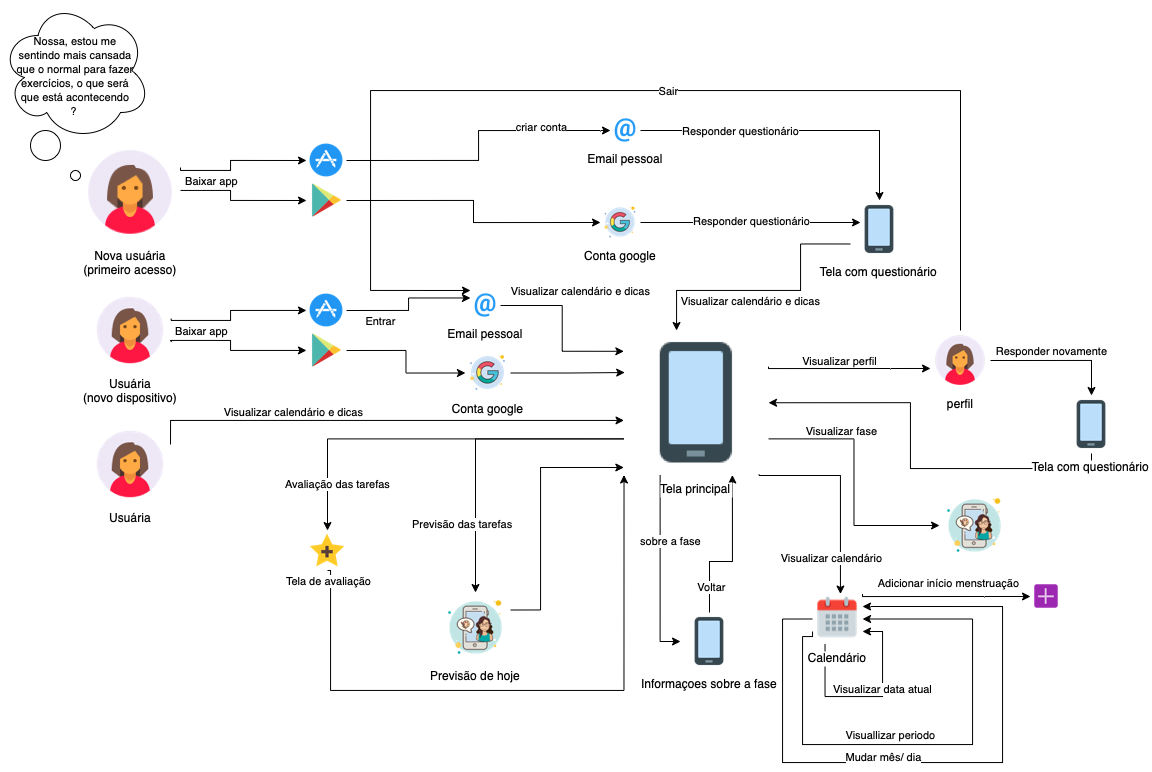
\includegraphics[keepaspectratio=true,scale=0.37]{figuras/richPicture.png}
	\end{center}
	\legend{Fonte: Autora}
    \label{fig08}
\end{figure}

A usuária, após fazer o cadastro, responde a um pequeno 
questionário para coletas iniciais de dados. Isso ajuda a reduzir 
o problema do começo frio, e fornece informações importantes
como data da última menstruação e quanto tempo dura a menstruação.

A data da última menstruação é importante para utilizar o 
método do calendário, descrito no referencial teórico (Capítulo \ref{ch:referencial}). 
Esse método é o que foi utilizado para determinar em que 
fase do ciclo a usuária se encontra.

\subsection{Protótipo de Alta Fidelidade}

O protótipo de alta fidelidade, desenvolvido no Figma, conta com a apresentação 
inicial do aplicativo com a logo. Depois, a usuária 
pode escolher entre entrar em uma conta existente ou criar 
uma nova (vide Figura \ref{fig09}). Caso a pessoa crie uma conta 
nova, ela será 
redirecionada ao questionário (vide Figura \ref{fig09}), e após 
respondido, a 
tela principal aparecerá (vide Figura \ref{fig10}). A tela inicial informa que 
fase do ciclo a pessoa está, qual o dia 
e qual o período. Através dessa tela, é possível acessar 
a tela de previsão das tarefas (vide Figura \ref{fig10}), de perfil
e uma página informativa (vide Figura \ref{fig11}).

\begin{figure}[ht]
	\caption{Protótipo - Entrar, Criar Conta e Questionário}
	\begin{center}
	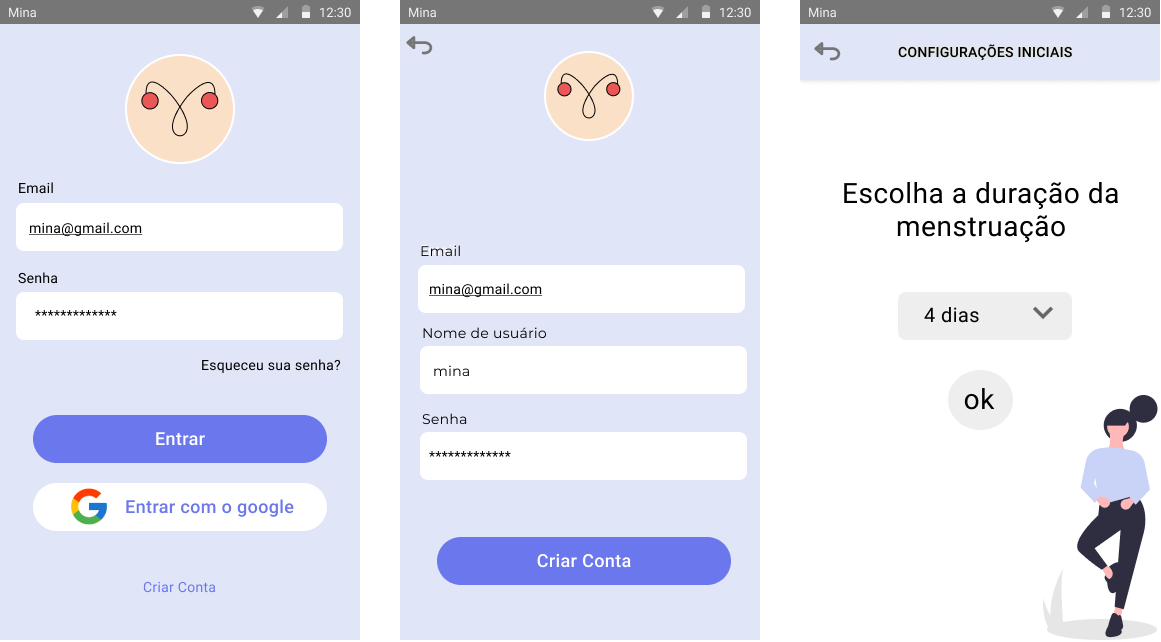
\includegraphics[keepaspectratio=true,scale=0.3]{figuras/prototipo1-v.png}
	\end{center}
	\legend{Fonte: Autora}
    \label{fig09}
\end{figure}

\begin{figure}[ht]
	\caption{Protótipo - Página Principal, Sobre a Fase e Adicionar Ciclo}
	\begin{center}
	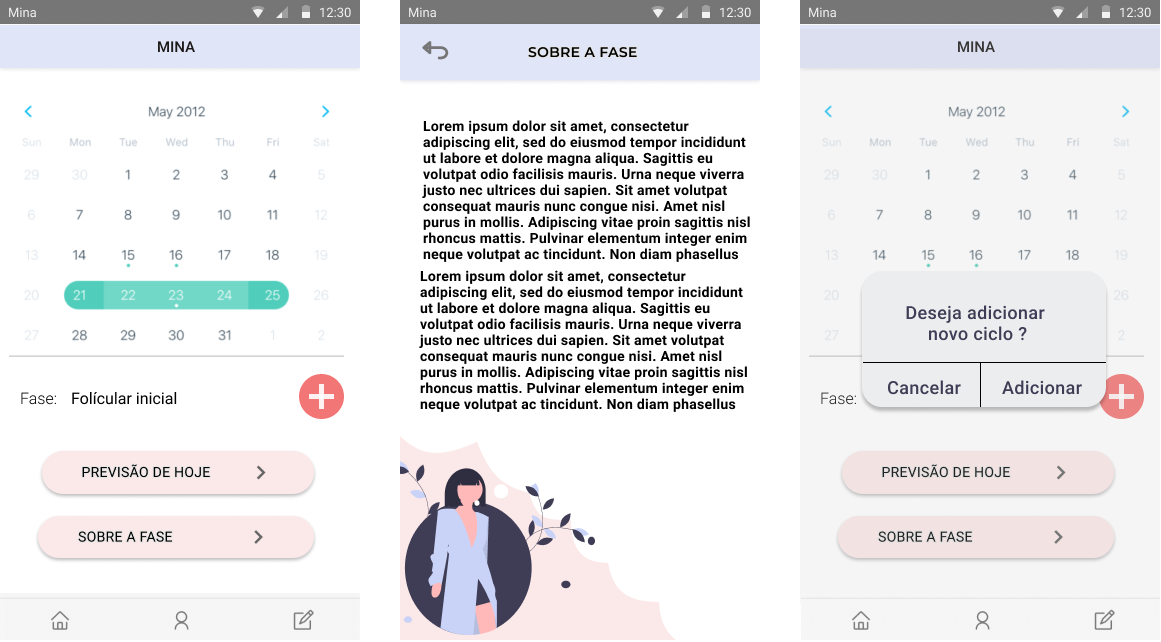
\includegraphics[keepaspectratio=true,scale=0.3]{figuras/prototipo2-v.png}
	\end{center}
	\legend{Fonte: Autora}
    \label{fig10}
\end{figure}

\begin{figure}[ht]
	\caption{Protótipo - Avaliação, Previsão e Perfil}
	\begin{center}
	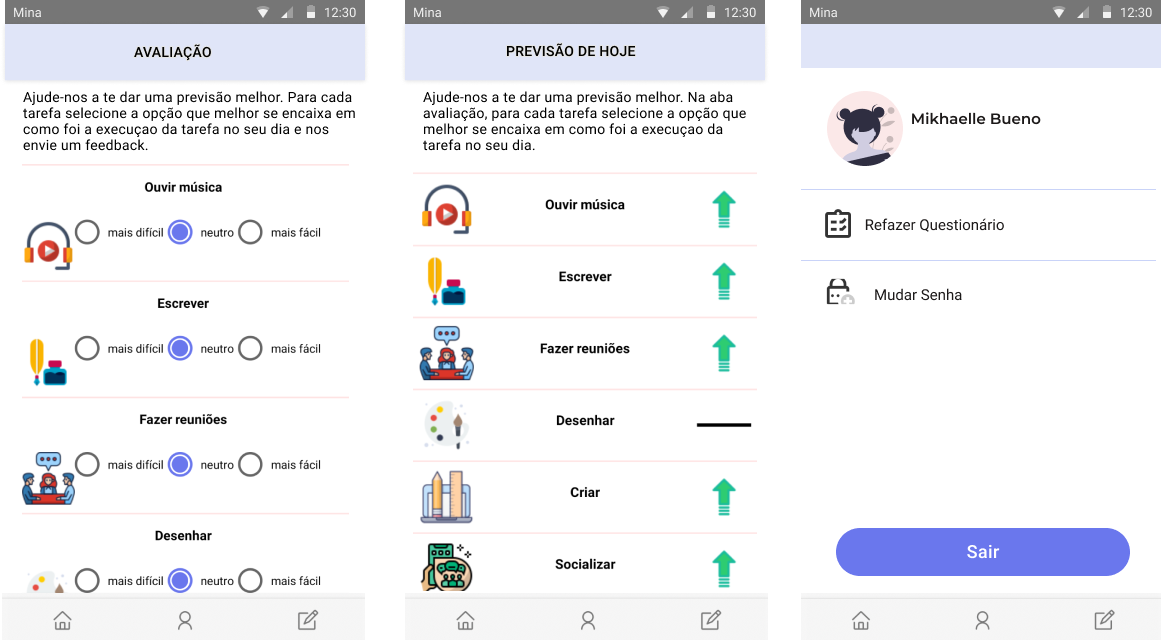
\includegraphics[keepaspectratio=true,scale=0.3]{figuras/prototipo3-v.png}
	\end{center}
	\legend{Fonte: Autora}
    \label{fig11}
\end{figure}

\section{Arquitetura}
\label{arq}

O aplicativo é construído com o \emph{framework} React Native, que gera aplicativos nativos Android e IOS. 
Ele se comunica com o Firebase Authentication, o qual fornece serviços \emph{backend} para autenticar 
o usuário no aplicativo. O Firebase Authentication suporta 
autenticação usando senhas, números de telefone, provedores de identidade como Google, Facebook, Twitter e 
outros. Na Aplicação, é utilizado para criação de usuário através de e-mail e senha ou 
pelo Google \emph{sing-in}. A Figura \ref{fig12} ilustra esses participantes.

As credenciais são armazenadas no Firebase, sendo utilizadas para realizar o 
\emph{login} e a recuperação de senha. Para cada usuário, é gerado um \emph{token} e um número único, chamado uid, permitindo 
fazer requisições seguras para as funções existentes na \emph{Cloud Functions}, que checam se as credenciais 
são existentes e válidas.

As funções do \emph{Cloud Functions} são responsáveis por executarem regras de negócio e 
pela comunicação com a base de dados \emph{Firestore}, lendo, inserindo e atualizando os dados. 
O Firestore é um banco de dados em nuvem NoSQL, flexível e escalável, para armazenar e sincronizar dados.
Uma vantagem de utilizar essa arquitetura é que utilizando a própria chave do usuário para identificar 
dados únicos nas tabelas, os acessos ficam rápidos e seguros, e a aplicação do \emph{React Native} reconhece 
através de \emph{listeners} que houve mudança nos dados do usuário, atualizando a aplicação em tempo real.
 
\begin{figure}[ht]
	\caption{Visão Arquitetural em Macro Nível}
	\begin{center}
	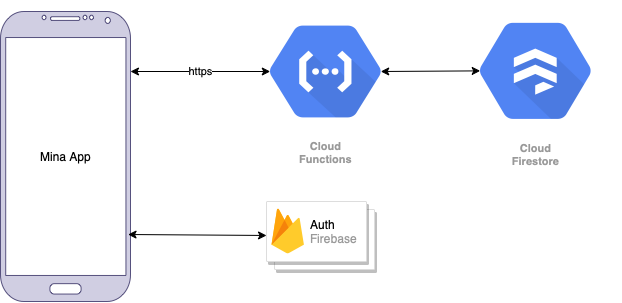
\includegraphics[keepaspectratio=true,scale=0.6]{figuras/architecture.png}
	\end{center}
	\legend{Fonte: Autora}
    \label{fig12}
\end{figure}

\subsection{Arquitetura \emph{Frontend}}

Na Figura \ref{fig13}, tem-se a organização da pasta do projeto \emph{frontend}. No \emph{React Native}, fora 
da pasta \emph{src}, tem o arquivo \emph{index.js}, que inicializa o aplicativo chamando do \emph{App.tsx}. 
O \emph{App.tsx} é responsável 
por criar as rotas de navegação e inicializar os contextos. Os \emph{contexts} são utilizados 
para compartilhamento, 
persistência de dados e comunicação com os \emph{services}. Os \emph{services} são responsáveis pela 
comunicação com 
os serviços externos.Nesse caso, com as funções do \emph{Cloud Functions}. As \emph{scenes} são as 
telas propriamente ditas, 
que consomem os dados do contexto e componentes reutilizáveis da pasta \emph{components}. 
Nos \emph{assets}, ficam as imagens, e 
nos \emph{managers} arquivos gerais de configuração. 

\begin{figure}[ht]
	\caption{Visão Arquitetural \emph{Frontend}}
	\begin{center}
	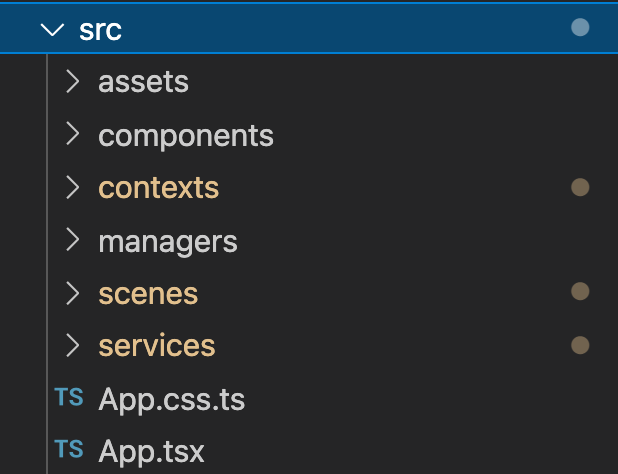
\includegraphics[keepaspectratio=true,scale=0.6]{figuras/frontend.png}
	\end{center}
	\legend{Fonte: Autora}
    \label{fig13}
\end{figure}

\subsection{Arquitetura \emph{Backend}}

A aplicação também se comunica com o serviço \emph{backend} \emph{Cloud Functions} através de requisições HTTPS.
O \emph{Cloud Functions} permite executar automaticamente o código de \emph{backend} em resposta a 
eventos acionados por recursos do Firebase e solicitações HTTPS. 
O código é armazenado na nuvem do Google, e executado em um ambiente gerenciado, caracterizando 
uma arquitetura \emph{serveless}, em que não há necessidade de gerenciar e dimensionar seus 
próprios servidores. 

\begin{figure}[ht]
	\caption{Funções na \emph{Cloud Functions}}
	\begin{center}
	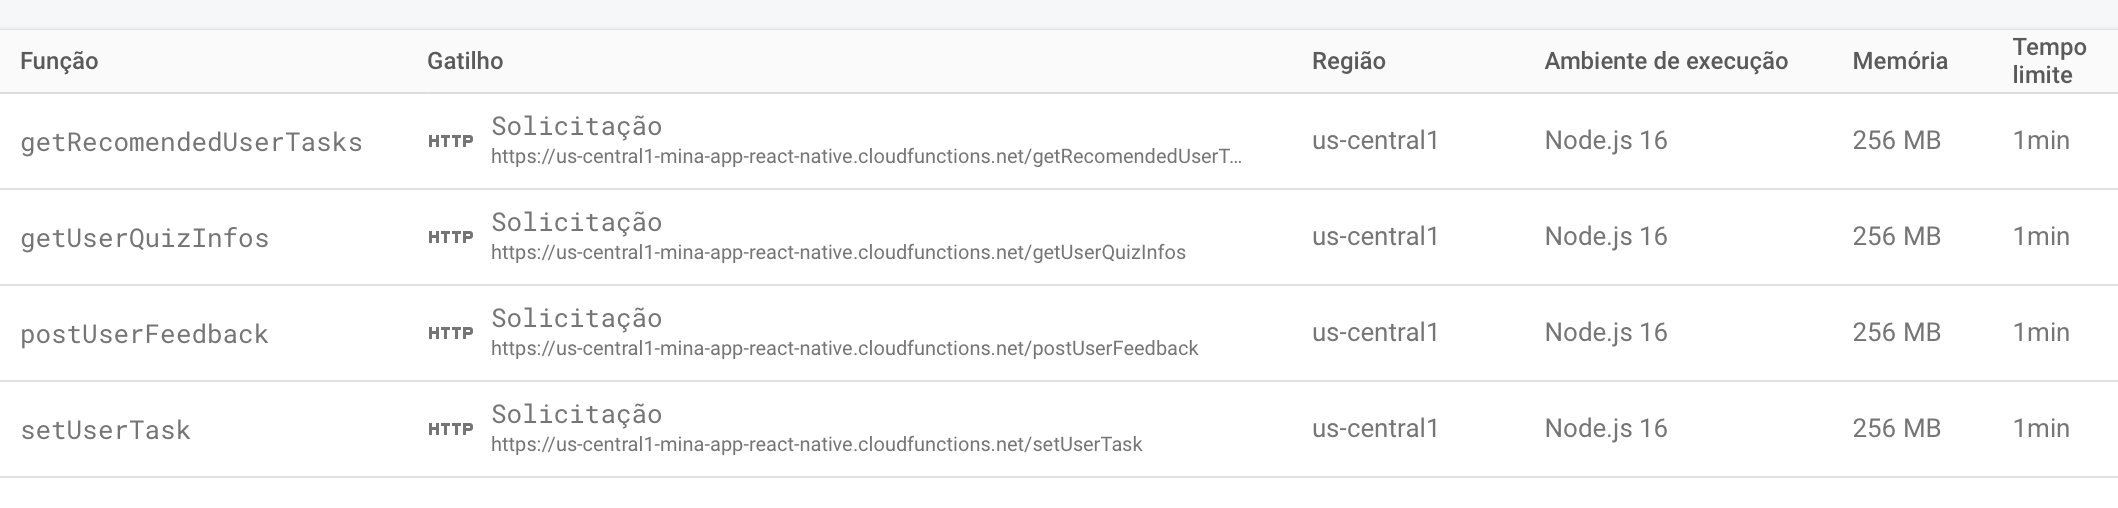
\includegraphics[keepaspectratio=true,scale=0.42]{figuras/funcoes.png}
	\end{center}
	\legend{Fonte: Autora}
    \label{fig14}
\end{figure}

\subsection{Sistema de Recomendação}
\label{sr}

A função \emph{postUserFeedback} (vide Figura \ref{fig14}) é responsável por conter o sistema de 
recomendação que atualiza o grupo ao qual o usuário está mais próximo, bem como atualiza os dados do usuário. 

A Figura \ref{fig15} representa a lógica em mais alto nível de como funciona essa função. Ela recebe 
um \emph{array} do \emph{frontend} com o \emph{feedback} enviado pelo usuário e qual fase o usuário se encontra. 
Depois, coleta os dados dos grupos e do usuário do banco de dados, selecionando os dados correspondentes à fase 
do usuário; soma os pontos aos tipos das tarefas avaliadas pelo usuário; compara os dados das tarefas do usuário 
com os dados dos grupos; calcula o número de inversões para cada grupo; seleciona o grupo com menor 
número de inversões; avalia se é o primeiro \emph{feedback} do usuário (se sim, adiciona as pontuações do usuário ao grupo correspondente) 
(caso contrário, avalia se houve mudança no grupo). Em havendo mudança, remove os pontos do usuário do grupo antigo e adiciona ao grupo novo. 

\begin{figure}[ht]
	\caption{Lógica em Alto Nível da Função \emph{postUserFeedback }}
	\begin{center}
	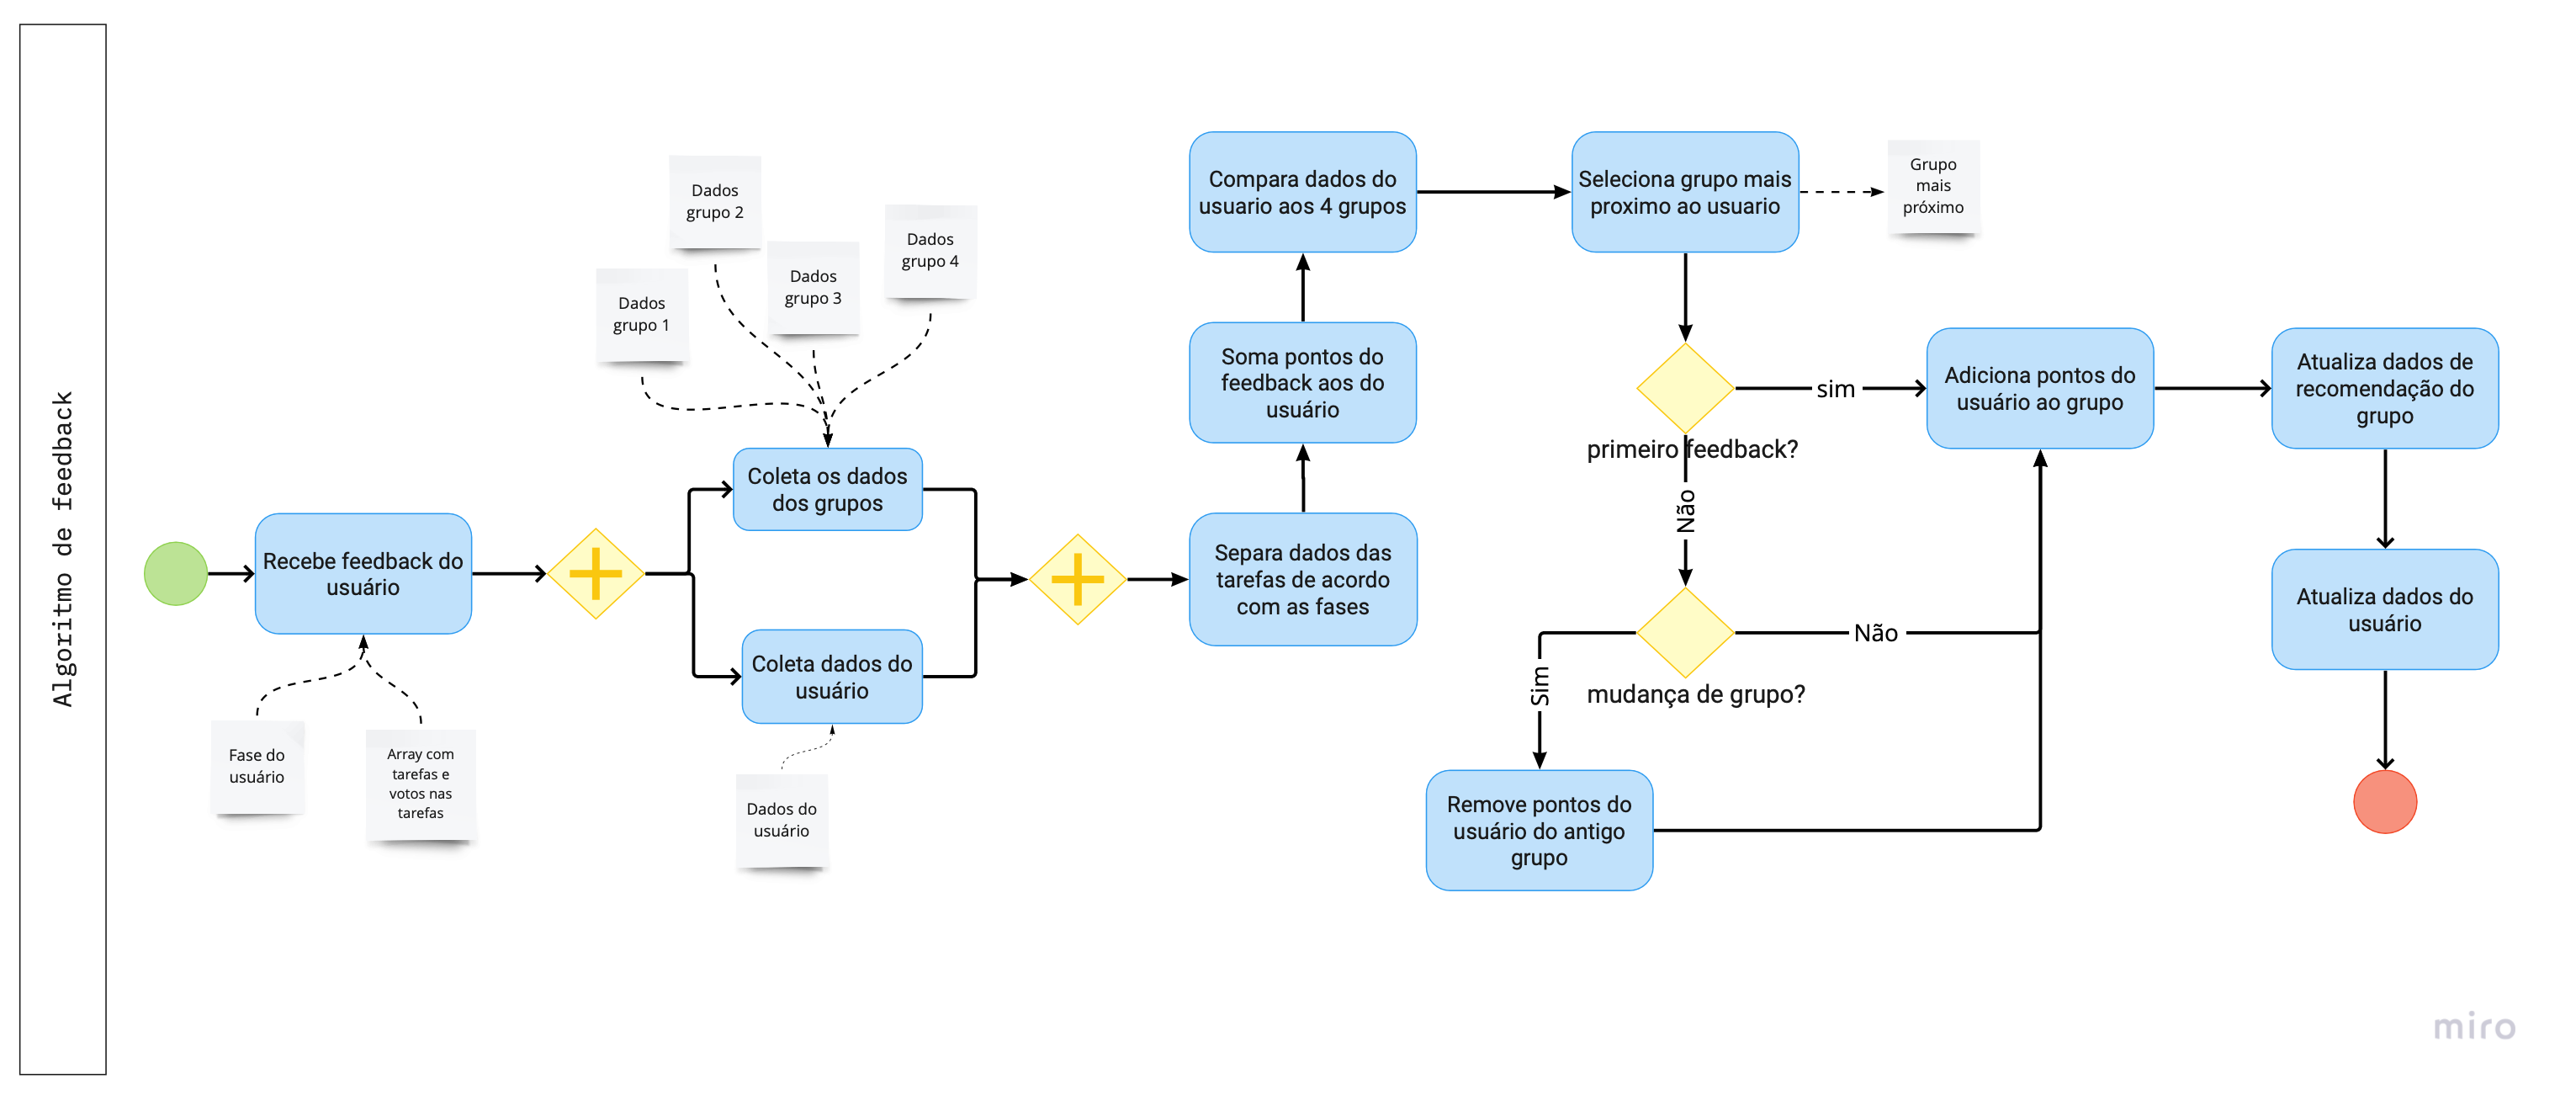
\includegraphics[keepaspectratio=true,scale=0.14]{figuras/recomendacao.png}
	\end{center}
	\legend{Fonte: Autora}
    \label{fig15}
\end{figure}

O sistema de recomendação utiliza um algoritmo chamado contagem de inversão. 
Dado um \emph{array} x com x[n] elementos, a contagem de inversão conta o quão longe o \emph{array} x está de ficar 
ordenado. Se o \emph{array} está ordenado, então, a contagem é 0. Se o \emph{array} está invertido, 
então, a contagem é máxima. Ou seja, dado dois elementos, x[i] e x[j], uma 
inversão ocorre se x[i] > x[j] e i<j.

A contagem de inversão foi aplicada no algoritmo utilizando a seguinte lógica. 
De 12 tarefas, para cada tarefa, 
há três possibilidades: ser mais fácil, neutra ou mais difícil. Para cada grupo, é montado um \emph{array} 
com as classificações das tarefas, por exemplo, exercitar - difícil, faxinar - neutro, socializar - fácil e assim 
sucessivamente para as 12 tarefas. A tarefa é considerada a posição do \emph{array} 
e o tipo dela o valor para comparação (Vide Figura \ref{fig16}).

\begin{figure}[ht]
	\caption{Função de Cálculo para a Fase}
	\begin{center}
	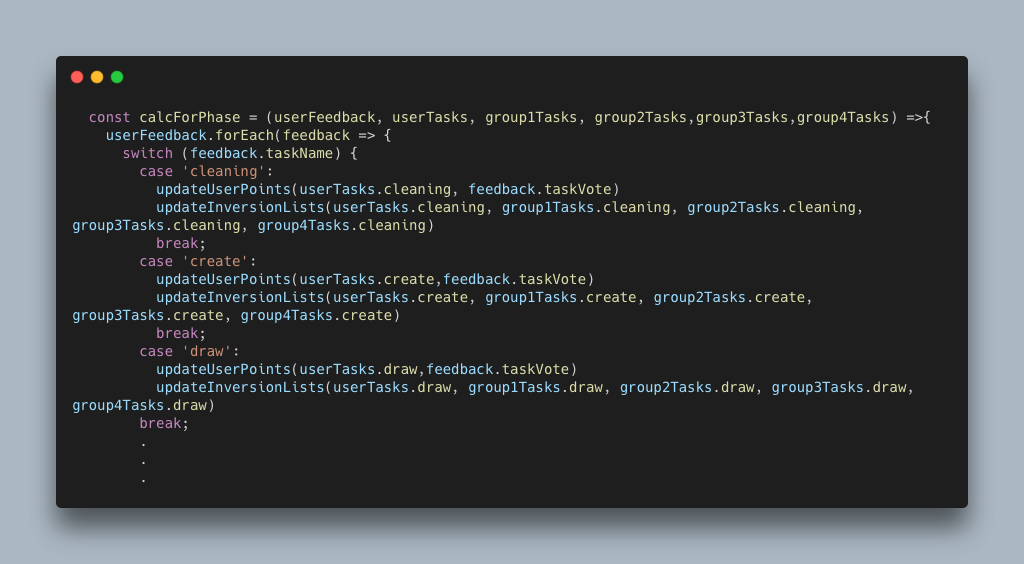
\includegraphics[keepaspectratio=true,scale=0.3]{figuras/code-calForPhase.png}
	\end{center}
	\legend{Fonte: Autora}
    \label{fig16}
\end{figure}

Da mesma forma, é montado um \emph{array} com os dados 
do usuário, por exemplo, exercitar - neutro, 
faxinar - fácil, socializar - difícil. O tipo mais votado da tarefa exercitar do usuário é comparado a com o da tarefa 
exercitar do grupo. 
Neste exemplo, é comparado neutro com fácil. Essa comparação gera uma inversão em relação ao grupo. 
Quando é comparado uma tarefa fácil com uma difícil, é contabilizado duas inversões (Vide Figura \ref{fig18}). 

\begin{figure}[ht]
	\caption{Função Para Contagem de Inversões}
	\begin{center}
	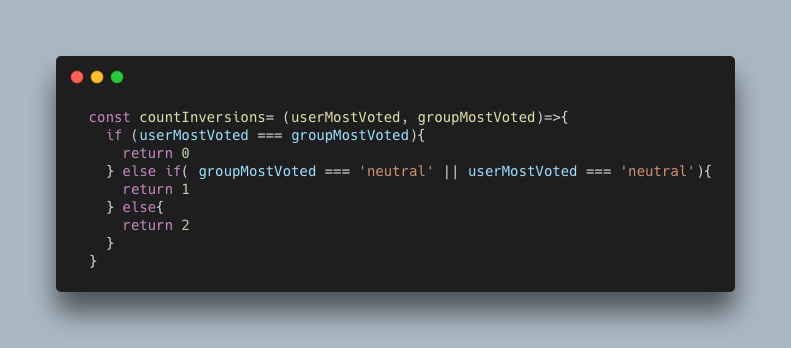
\includegraphics[keepaspectratio=true,scale=0.4]{figuras/code-countInversions.png}
	\end{center}
	\legend{Fonte: Autora}
    \label{fig18}
\end{figure}


Um \emph{array} com o número de inversões é então montado e, posteriormente, somado para ter o resultado final de qual grupo tem menor número de 
inversões em relação ao \emph{feedback} do usuário (Vide Figura \ref{fig17}). 
Para o caso dessa aplicação, que possui 12 tarefas, o número mínimo de inversão é 0 e o máximo é 24. Ao comparar os dados do usuário 
com os outros quatro grupos, o grupo com o menor número de inversões é atribuído ao usuário. 

\begin{figure}[ht]
	\caption{Função Para Atualizar \emph{Arrays} de Inversões}
	\begin{center}
	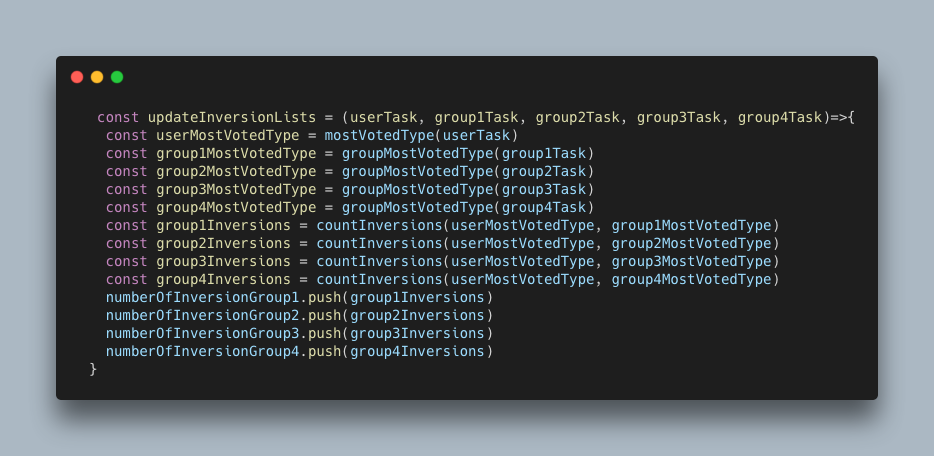
\includegraphics[keepaspectratio=true,scale=0.35]{figuras/code-updateInversionLists.png}
	\end{center}
	\legend{Fonte: Autora}
    \label{fig17}
\end{figure}

De acordo com as características descritas anteriormente, o sistema de recomendação é classificado como Colaborativo, por inserir o usuário a 
um grupo mais próximo, e fornecer a recomendação de acordo com os dados desse grupo. Além disso, ele também pode ser classificado como 
algoritmo baseado em memória, por utilizar classificações anteriores do usuário para um novo processamento.


\section{Aplicativo}

O aplicativo foi desenvolvido com sucesso, integrando todas as tecnologias citadas nas seções anteriores, e 
utilizando a metodologia de desenvolvimento estabelecida. Os requisitos acordados no Rich Picture Inicial, bem como no protótipo, também foram respeitados da forma
mais fiél possível.

Tiveram mudanças pontuais em comparação ao que foi estabelecido na primeira etapa do TCC. A tela de avaliação das tarefas e 
previsão foi separada com o intuito de melhorar a usabilidade, já que as funções das telas são diferentes.
Além disso, houve mudança na forma de inserção de um novo ciclo, agora, disponível em formato de calendário. 
Também foi retirada a parte de previsões de sintomas, já que o objetivo estabelecido é focado na recomendações de 
tarefas, e não em possíveis sintomas físicos ou mudanças de humor.

Na Figura \ref{fig19}, têm-se as telas de \emph{login} com senha e email; criação de conta com email, nome e senha; 
\emph{login} utilizando a conta Google, e redefinição de senha.

\begin{figure}[ht]
	\caption{\emph{Login}, Criação de Conta, Entrar com o Google e Redefinição de Senha}
	\begin{center}
	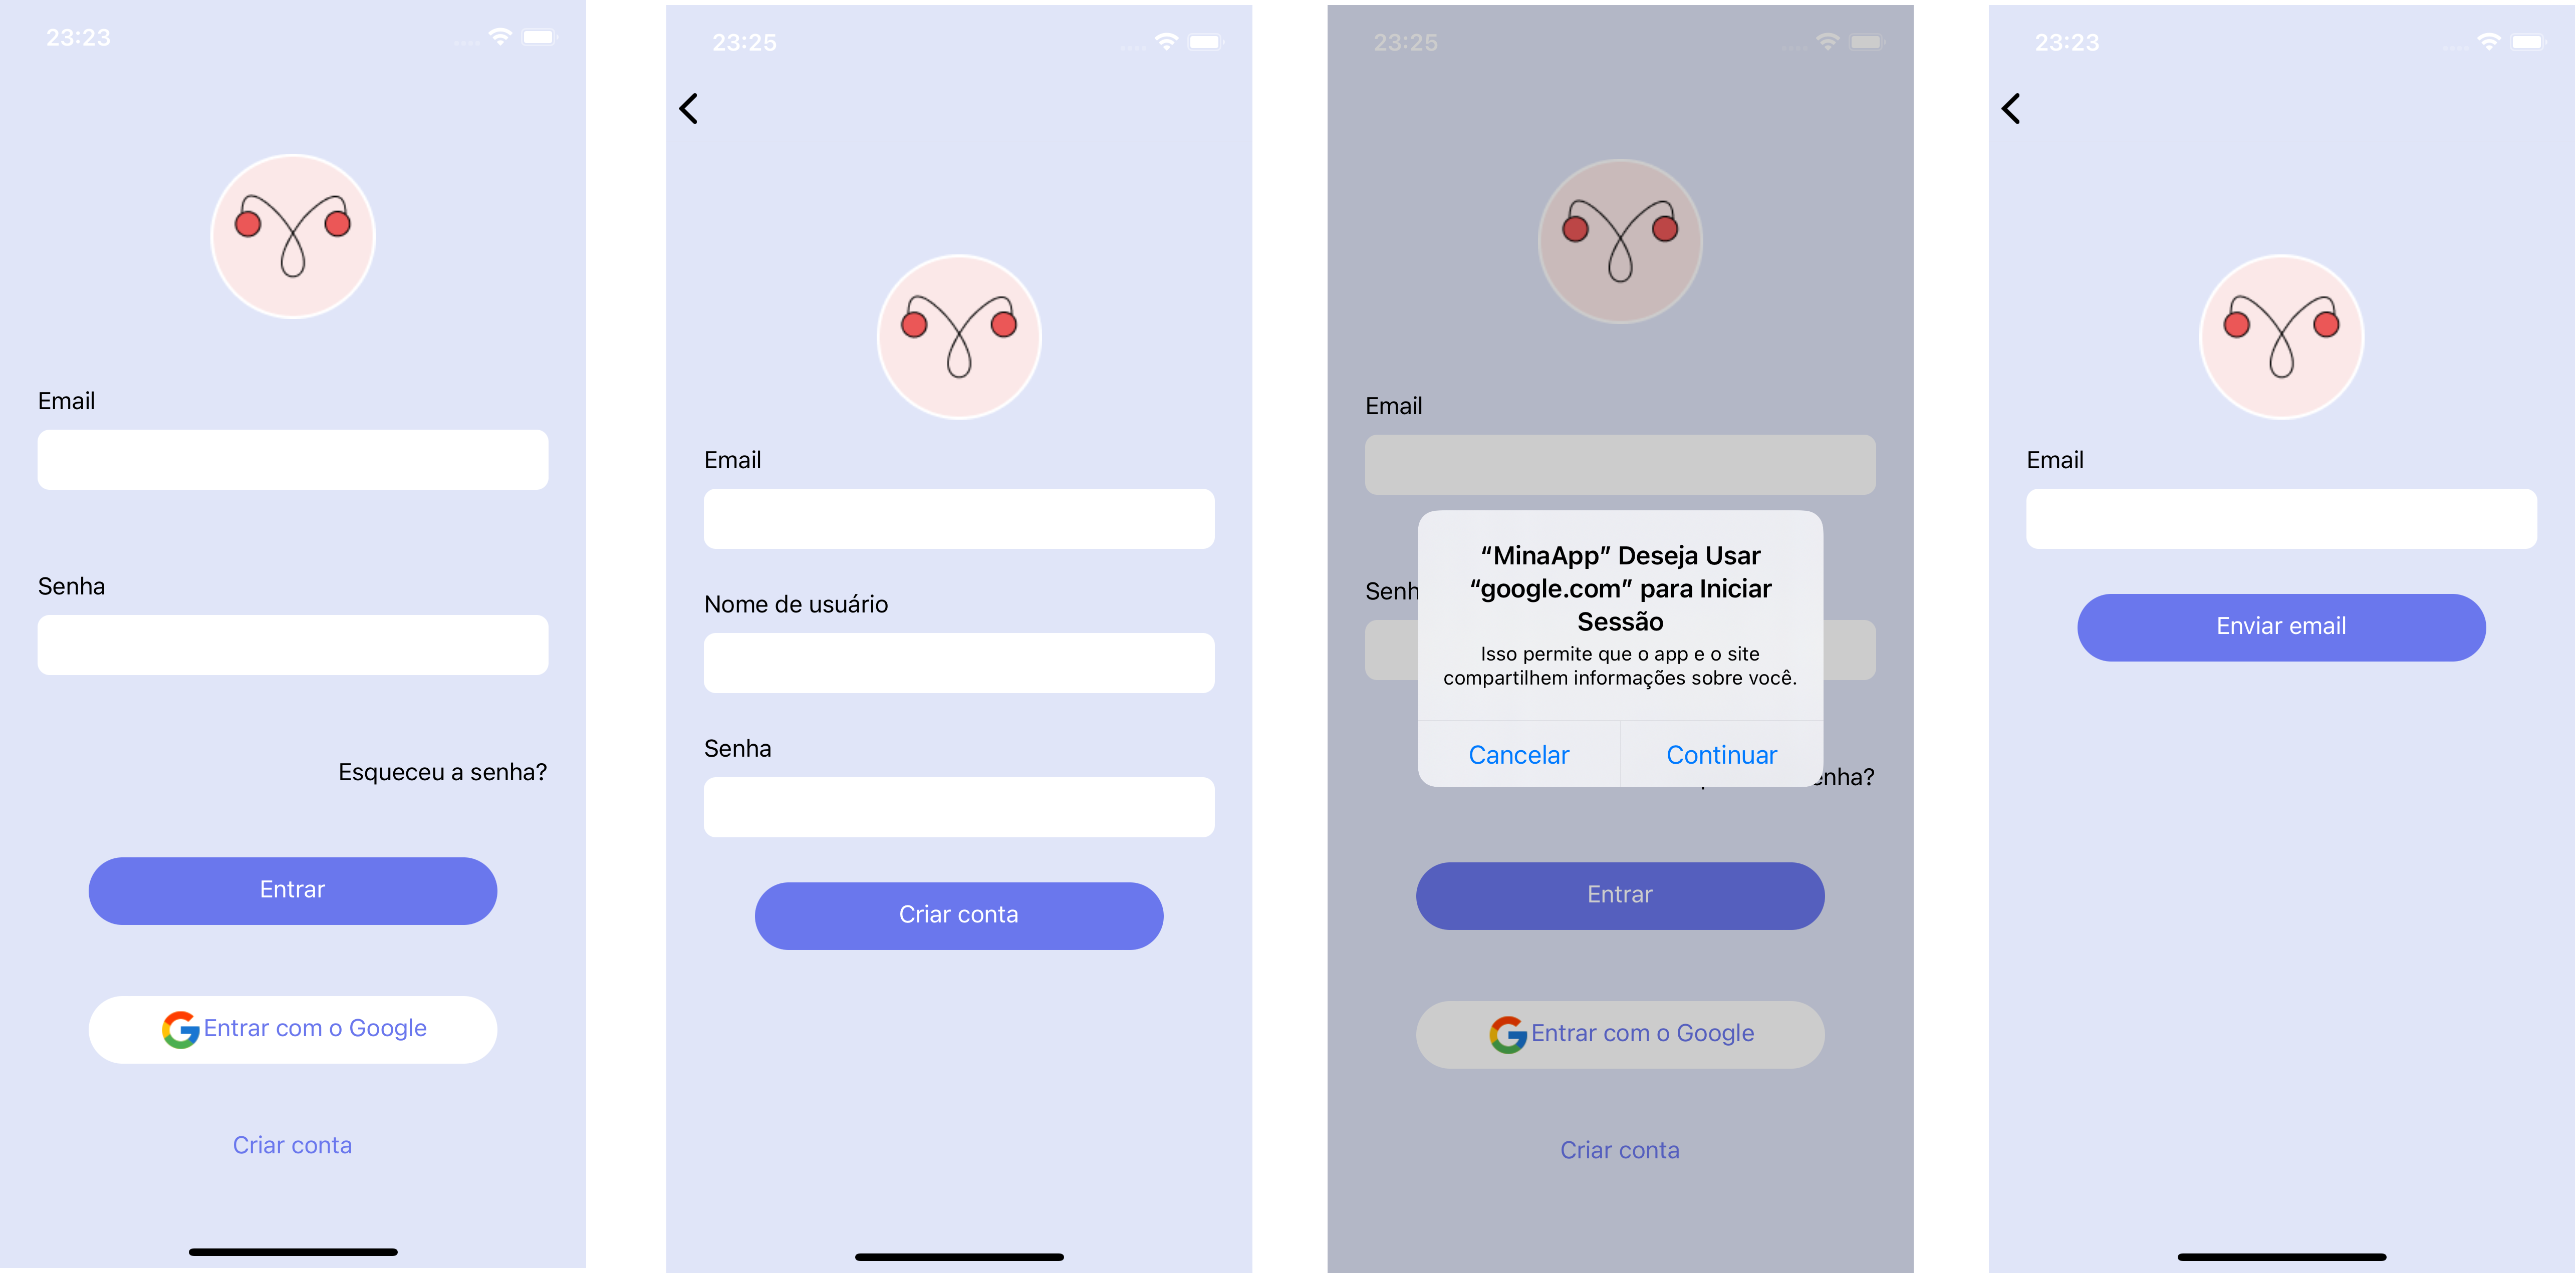
\includegraphics[keepaspectratio=true,scale=0.08]{figuras/aplicativo1.png}
	\end{center}
	\legend{Fonte: Autora}
    \label{fig19}
\end{figure}

Na Figura \ref{fig20}, têm-se as telas do questionário inicial. Ao todo, são seis perguntas; qual a data da sua 
última menstruação; quanto tempo dura normalmente sua menstruação?; quanto tempo dura normalmente seu ciclo?;
você considera seu ciclo regular? você utiliza métodos contraceptivos hormonais?; você tem algum distúrbio 
endócrino como ovário policísticos ou outros?, e você possui sintomas de tensão pré menstrual (TPM)? 
De acordo com as respostas, a usuária será inserida em um grupo inicial.

\begin{figure}[ht]
	\caption{Questionário Inicial}
	\begin{center}
	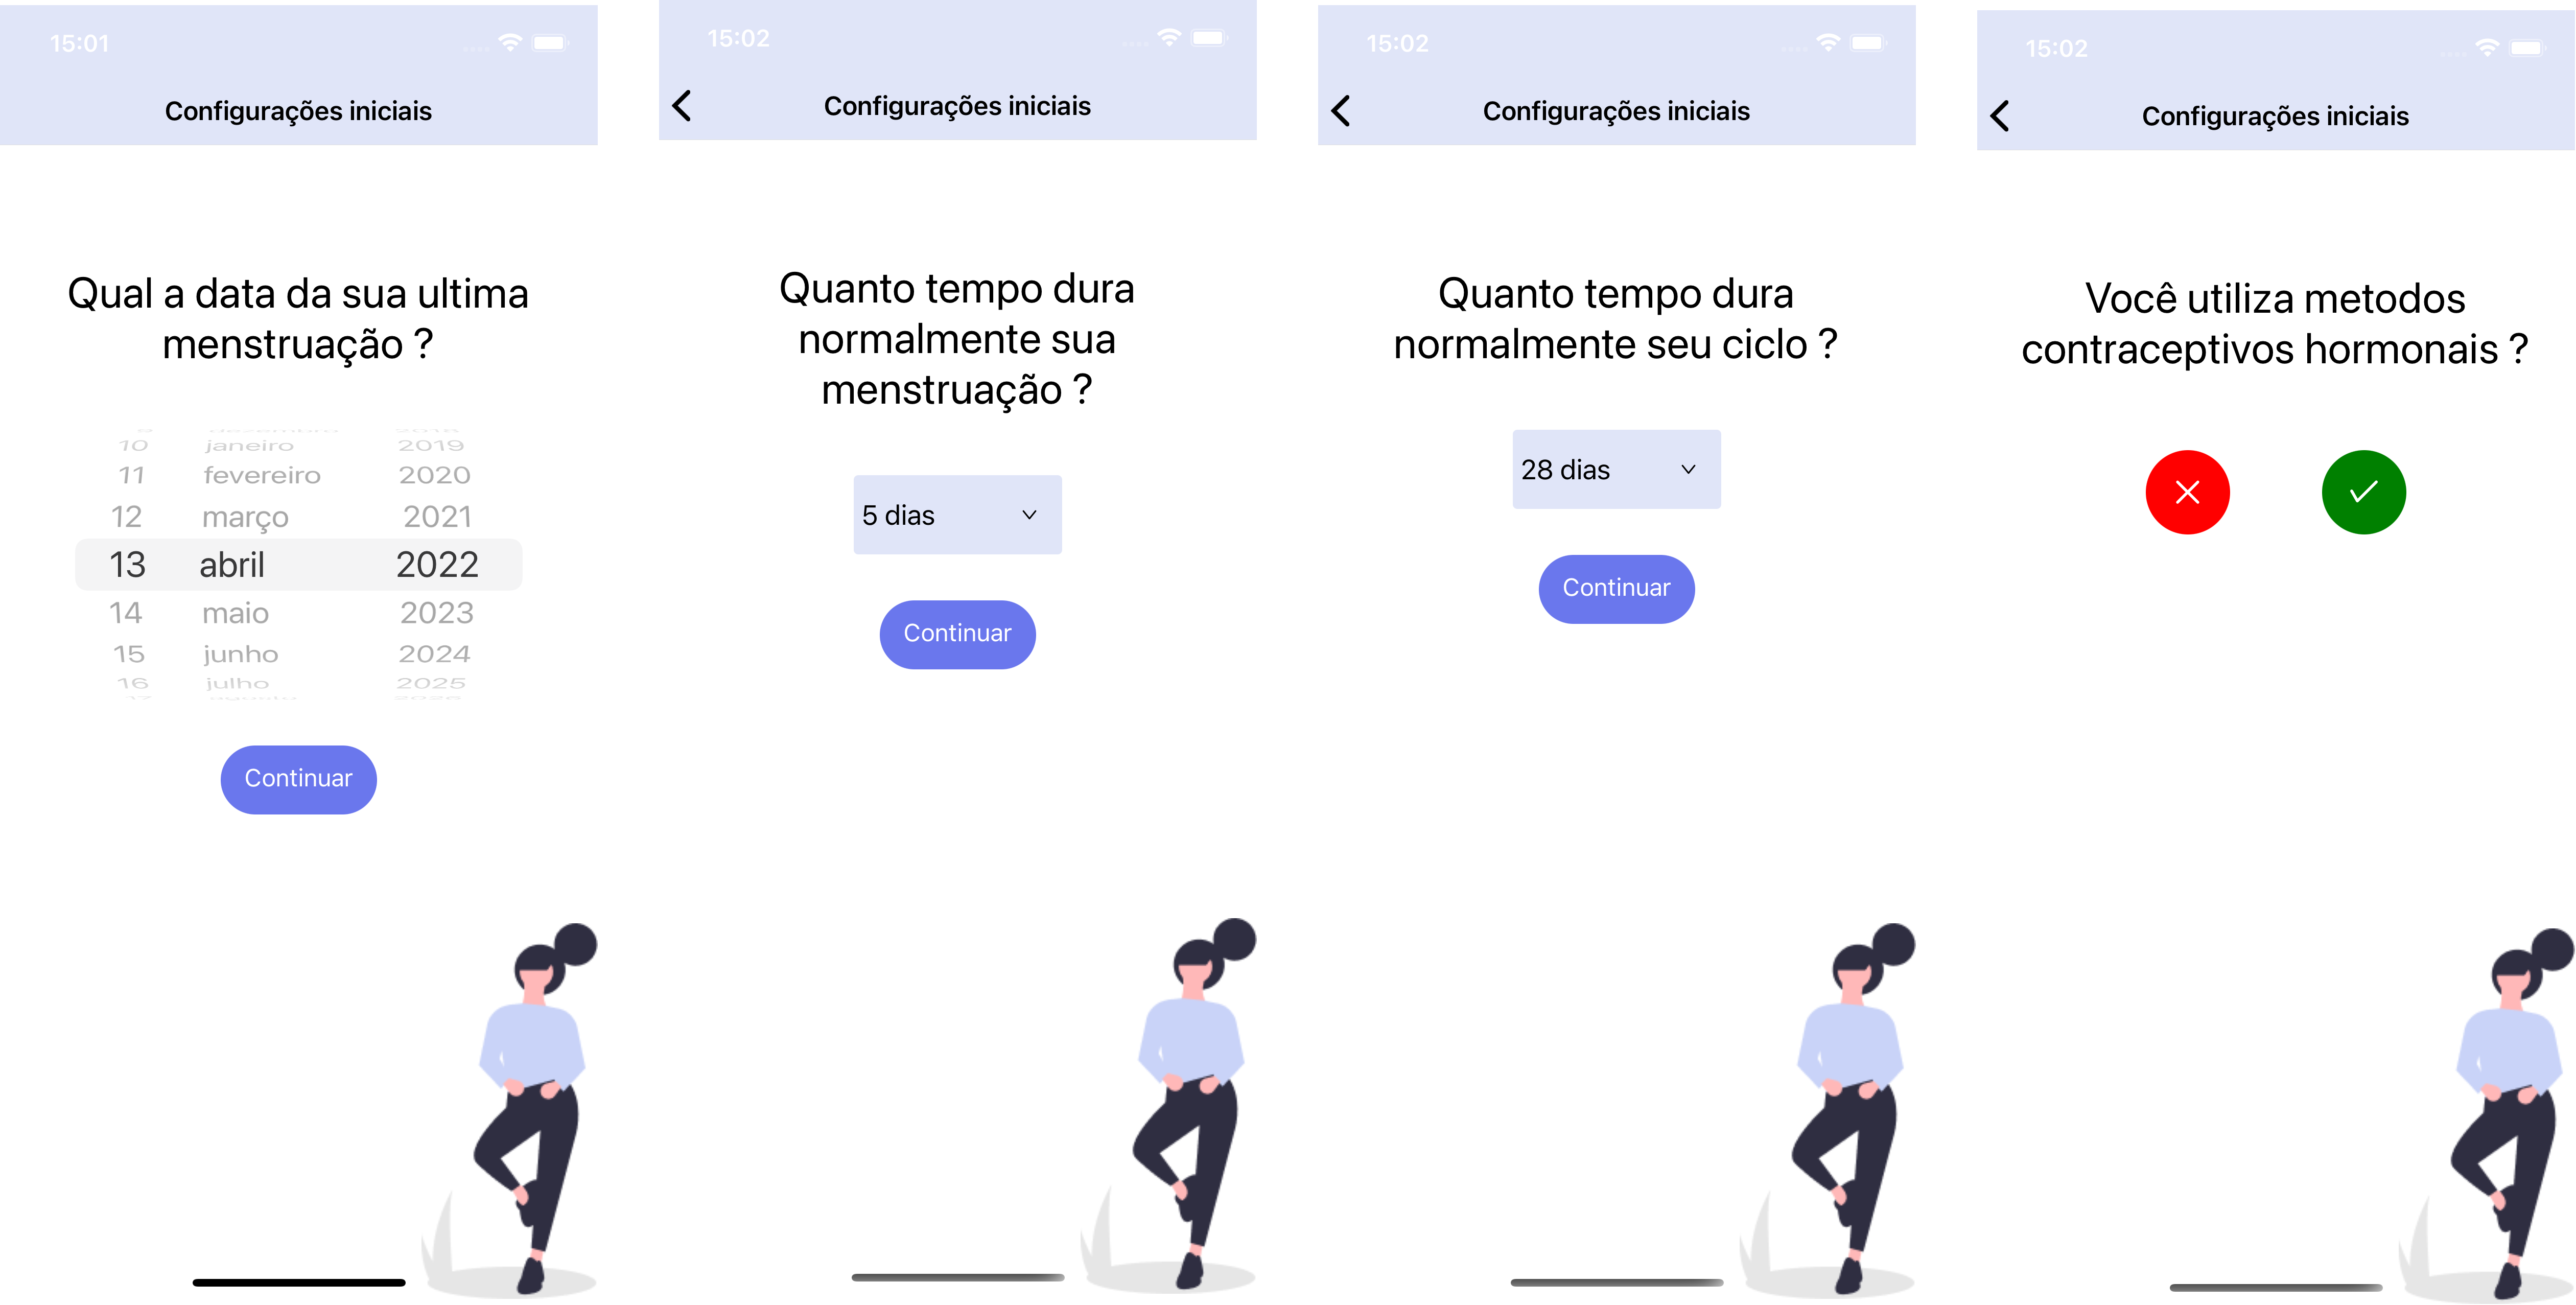
\includegraphics[keepaspectratio=true,scale=0.08]{figuras/aplicativo4.png}
	\end{center}
	\legend{Fonte: Autora}
    \label{fig20}
\end{figure}

Na Figura \ref{fig21}, têm-se as telas com o calendário que informa que fase do ciclo o usuário está através 
de um estímulo visual com as cores das bolas nas datas e através de um texto. É possível adicionar um novo ciclo 
clicando no '+', navegar entre as telas do menu, navegar para a tela com um texto sobre a fase e para a tela 
de recomendação de tarefas ou para o perfil. No perfil, é possível responder novamente o questionário ou 
realizar o \emph{logout}.

\begin{figure}[ht]
	\caption{Calendário, Adicionar Novo Ciclo, Sobre a Fase e Perfil}
	\begin{center}
	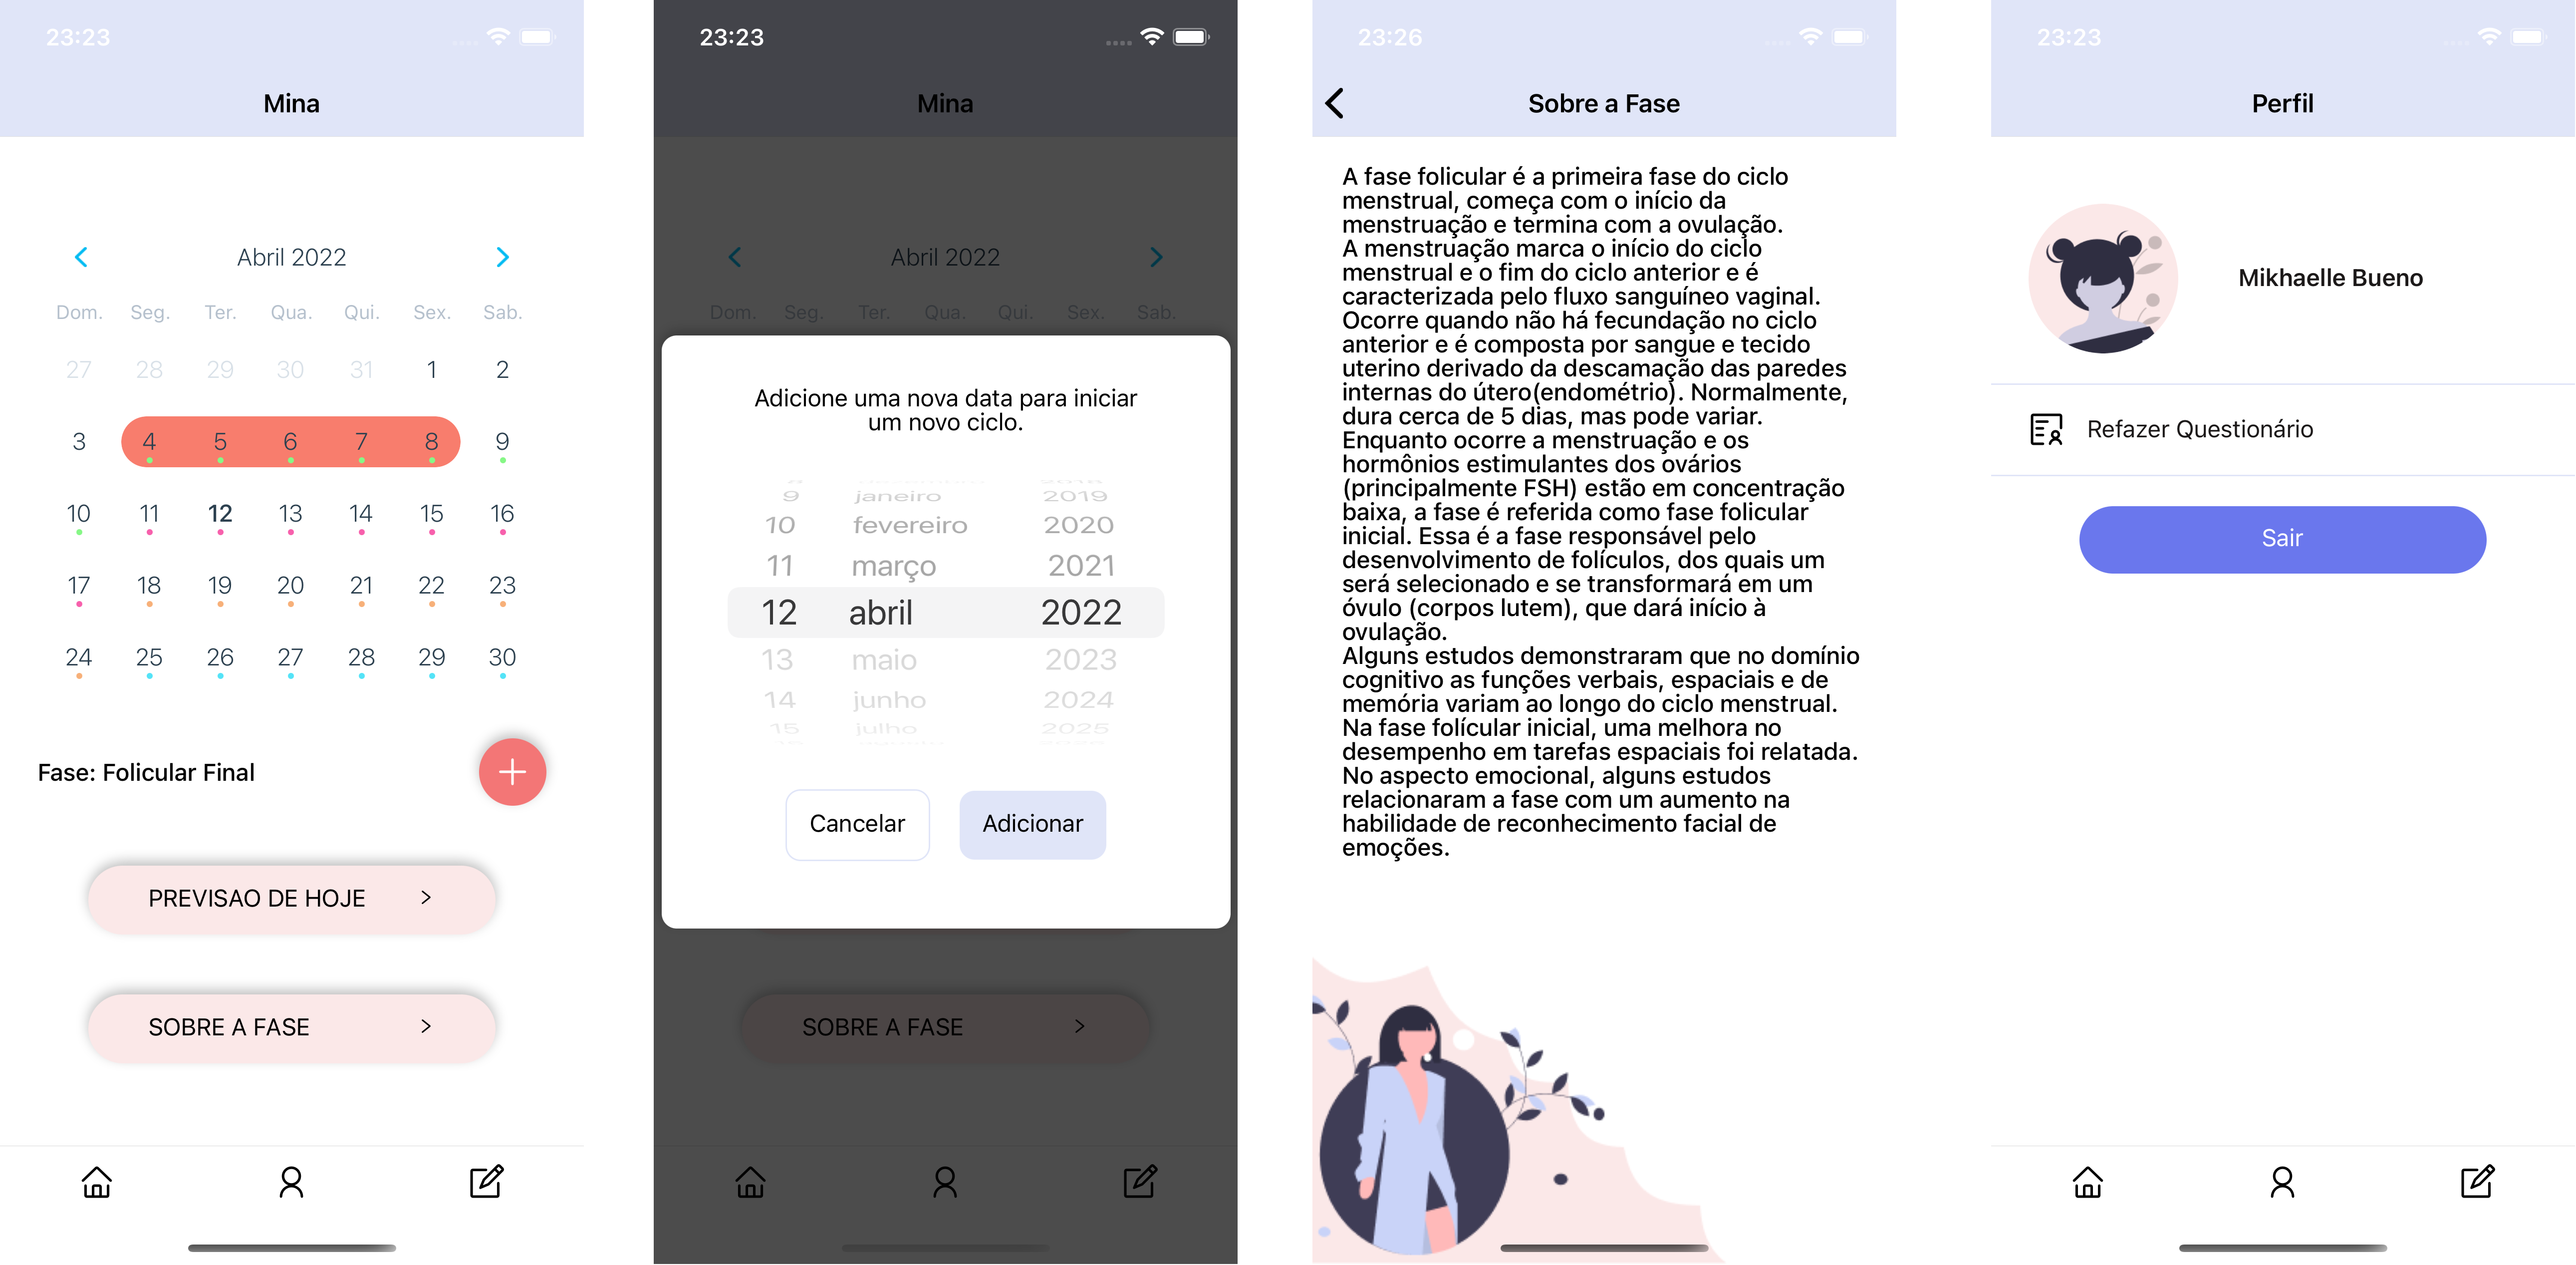
\includegraphics[keepaspectratio=true,scale=0.08]{figuras/aplicativo2.png}
	\end{center}
	\legend{Fonte: Autora}
    \label{fig21}
\end{figure}


Na Figura \ref{fig22}, têm-se as telas de previsão e avaliação. Na tela de avaliação, é possível enviar 
um \emph{feedback} com a avaliação do usuário para as tarefas de acordo com a fase do ciclo. Na tela de 
previsão, estão as recomendações dadas ao grupo que o usuário melhor se encaixa de acordo com o sistema de recomendação.
Enquanto o usuário não tiver enviado uma avaliação, a recomendação mostrada será do grupo atribuído quando o 
usuário respondeu ao questionário. É possível, 
após enviar as avaliações, que o usuário seja alocado para o grupo mais próximo.

\begin{figure}[ht]
	\caption{Tela de Avaliação e Previsão}
	\begin{center}
	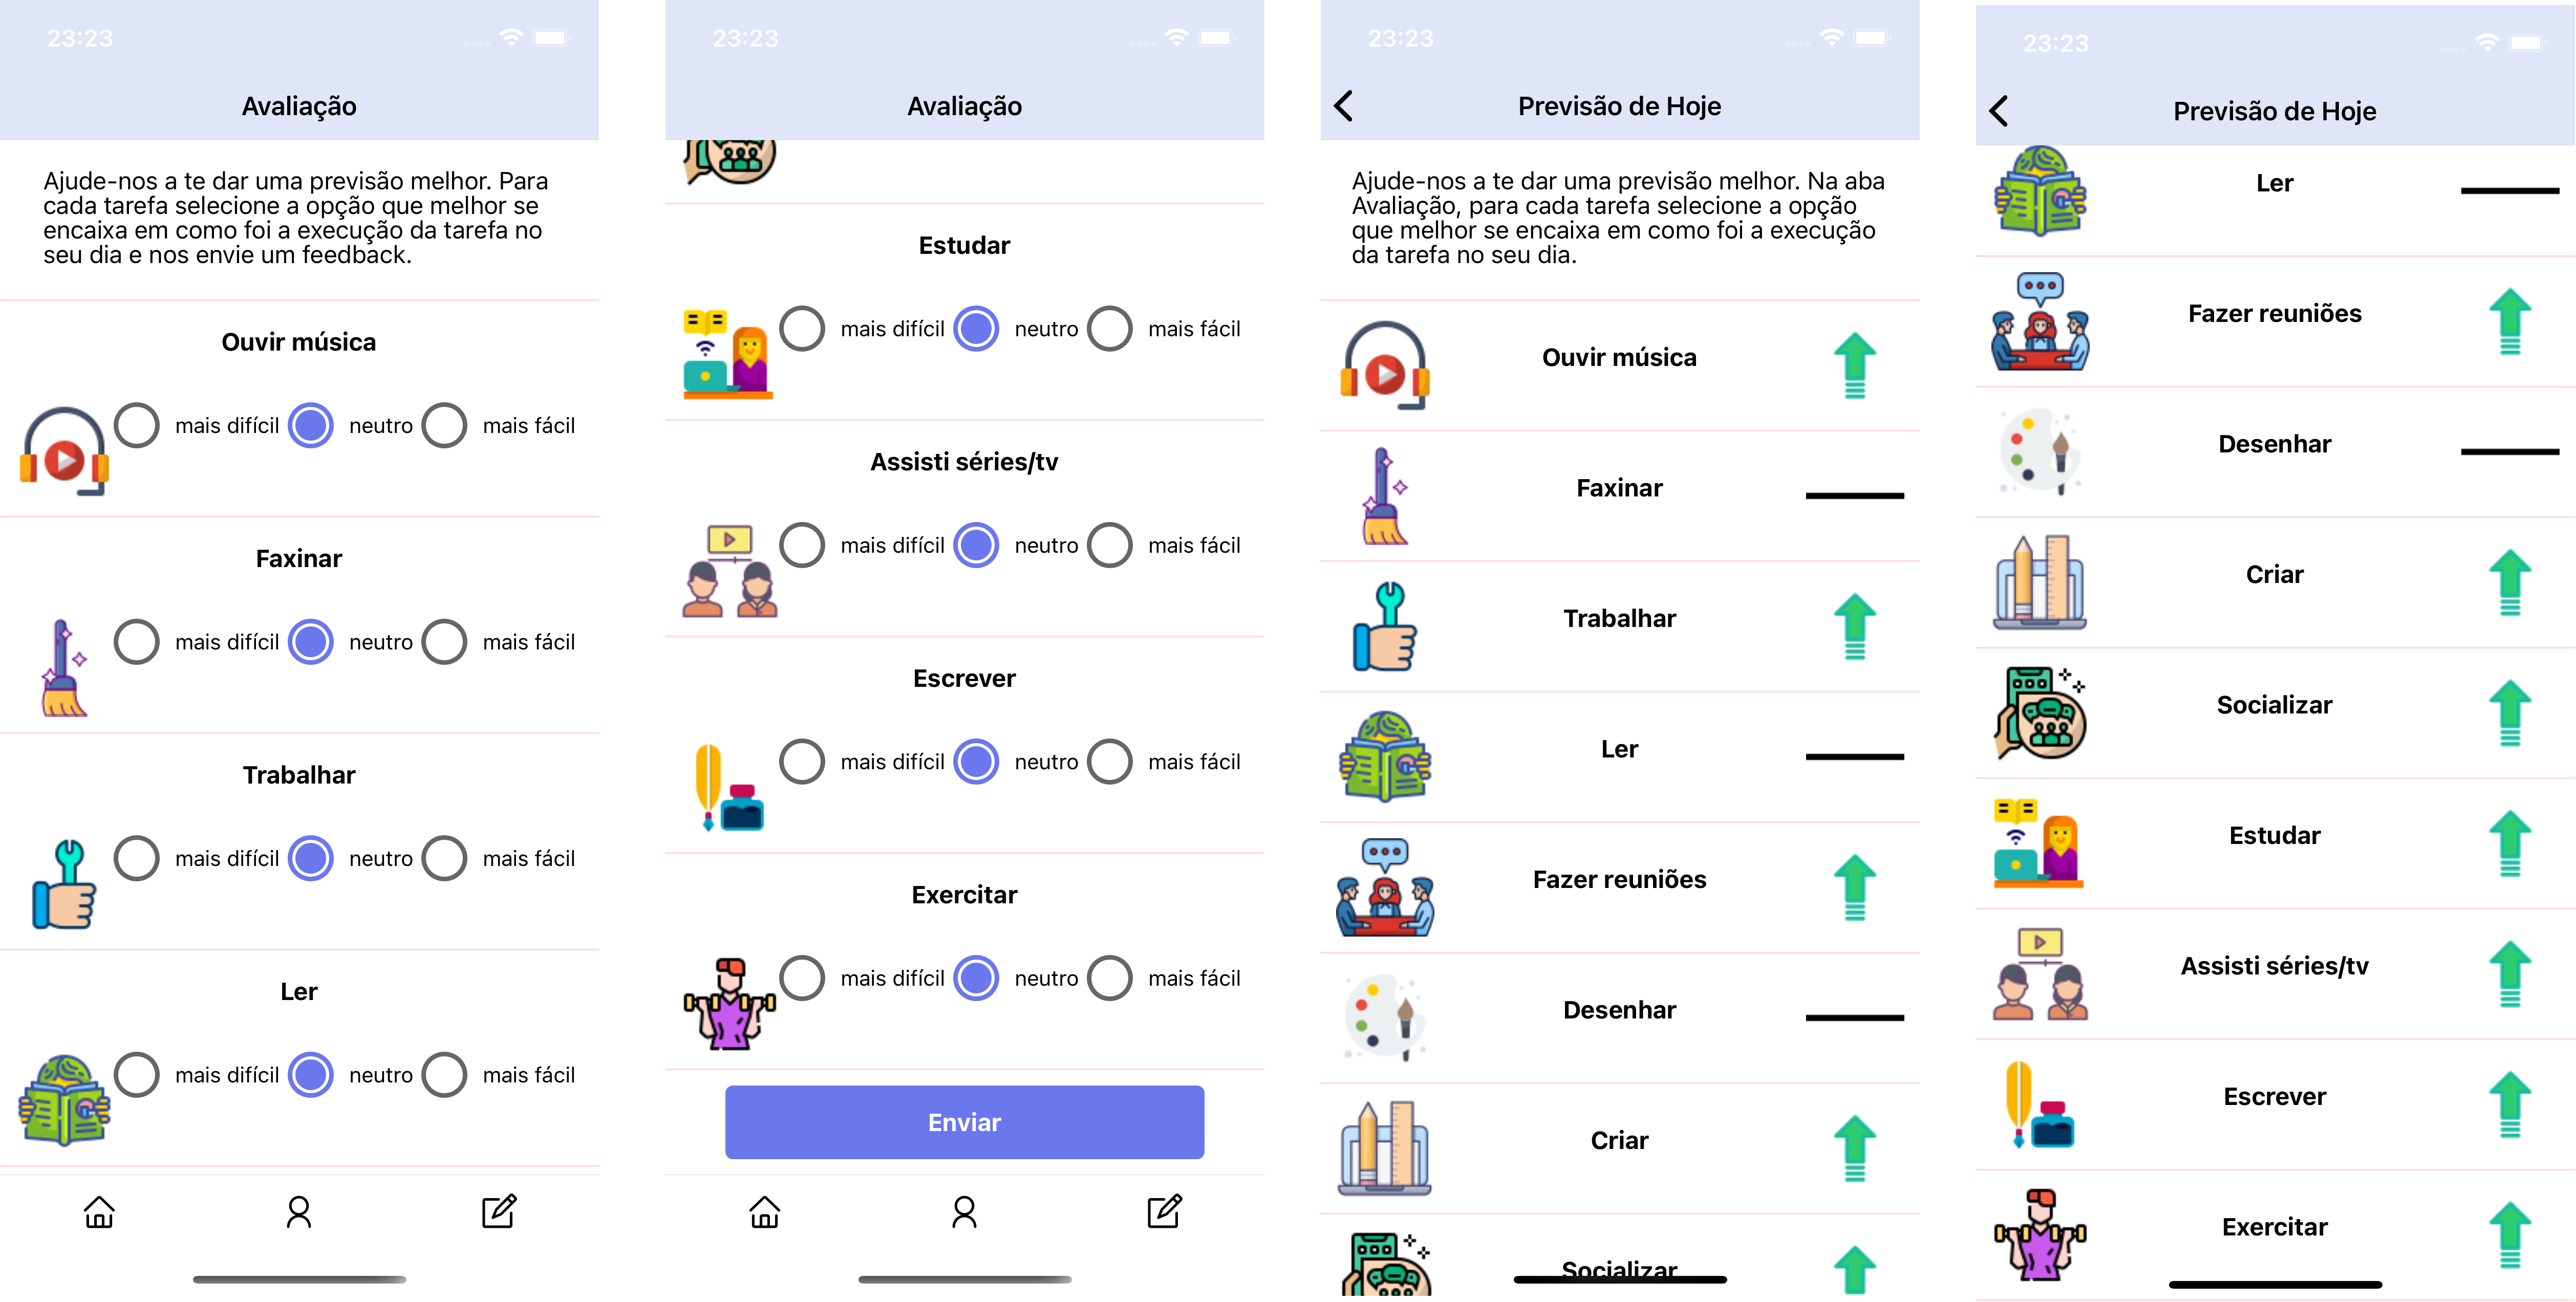
\includegraphics[keepaspectratio=true,scale=0.08]{figuras/aplicativo3.png}
	\end{center}
	\legend{Fonte: Autora}
    \label{fig22}
\end{figure}

Uma entrevista guiada por questionário foi feita para coletar o \emph{feedback} das usuárias, e a análise 
dos resultados será descrita no próximo capítulo. 


\section{Considerações Finais do Capítulo}

Neste capítulo, foi descrito o processo da tomada de decisão 
da ideia para 
esse trabalho, na seção de considerações iniciais. Na seção 
\ref{coletadados}, 
foi descrito o processo de definição do aplicativo como 
plataforma; o primeiro questionário, e o segundo questionário 
visando à coleta de dados. Na seção \ref{vsf2}, foram 
listados alguns perfis identificados 
com a análise de dados dos questionários, e classificadas as 
tarefas que demandam mais ou menos energia 
para serem executadas, de acordo com os grupos e as fases do ciclo menstrual. 
Esse processo levou em consideração 
as respostas dos questionários e a referência bibliográfica. 
A seção \ref{req} trouxe os requisitos elicitados, e o protótipo de alta fidelidade. 
Na seção \ref{arq}, foram descritos a arquitetura utilizada para desenvolvimento do 
\emph{frontend}, \emph{backend}, e como o algoritmo de recomendação funciona. Por último, 
mas não menos importante, consta o resultado final do aplicativo Mina com todas as \emph{features} 
implementadas.
